\chapter{Goal-oriented Dependability Analysis}\label{ch:proposal}

This chapter presents our proposed goal-oriented dependability analysis based on PMC applied to the MPERS case study. TROPOS early and late requirements phases are shortly presented - as TROPOS is the reference methodology for goal modelling and analysis, as well as the dependability verification that requires a behaviour specification - provided by the runtime goal model -  and the context effects specification - provided by the contextual goal model.

%Further details about the TROPOS methodology may be found in the reference literature~\cite{Bresciani:2004}. 


%from a goal model alternative selected for analysis of a given local or root goal 

Figure~\ref{fig:CRGM_TO_DTMC} illustrates the goal-oriented reliability analysis process that starts with conventional goal-oriented modelling and analysis phases of the TROPOS methodology and finishes with the generation of a high-level DTMC model used for reliability analysis. 

%Figure~\ref{fig:GODA_MODELS} presents the models involved in the analysis.

\begin{figure*}[h!]
\centering
\includegraphics[width=0.9\textwidth]{imgs/CRGM_TO_DTMC.png}
\caption{Goal-oriented dependability analysis activities.}
\label{fig:CRGM_TO_DTMC}
\end{figure*}

The next sections are structured as follows. First, a goal modelling and analysis as described by TROPOS methodology is performed~\cite{Bresciani:2004}. Next, the RGM behaviour rules are further explained and added to the MPERS goal model. Then, context notation is added to the RGM. After this, the high-level DTMC model for MPERS is built and details about the mapping of a RGM into a DTMC in PRISM language are provided, as well as the inclusion of the CGM context effects. Next, PCTL properties representing the reliability of fulfilling different system goals are defined. Finally, we demonstrate how our verification approach may be employed in reliability analysis. 


\section{Mobile Personal Emergency Response System}

The MPERS case study will be further detailed in later sections as the proposed goal-oriented reliability analysis based on PMC is described using the MPERS goal models created at the requirements engineering phases of TROPOS methodology. As such, this section will be limited to cover some relevant aspects of this system that justify the use of our formal verification approach to analyse its reliability.

An emergency response system is a mission-critical system for which failures in achieving its main goals by the time they are required may lead to catastrophic consequences on users, i.e., on individuals monitored by the system expecting to be promptly assisted in case of a medical emergency. Accordingly, any stakeholder that wishes to offer a service based on this system will have both ethical and contractual obligations regarding the safety of its product, that is, it must employ all means to prevent system failures and to attain dependability.

MPERS is expected to have a high availability - as it must be ready to respond to an emergency that may happen at any time - and a high reliability - as an incorrect emergency response may lead to death or to costly false-positives. Integrity is a less critical attribute in this case, but it must also be addressed as user's privacy may not be violated by disclosing his personal health or geolocation information to unauthorized persons. Maintainability is addressed, among others, by the use of a software development methodology and by the ability to update emergency rules remotely at runtime.

Environment changes is an important factor for MPERS, as the following conditions may change:

\begin{itemize}

\item The battery of the mobile device;
\medskip

\item The battery of the vital signs sensors;
\medskip

\item The disc memory used for storing the vital signs history;

\item The mobile signal used for data communication and for geolocation triangulation;
\medskip

\item The GPS signal used for geolocation;
\medskip

\item The health risk of the patient;
\medskip

\end{itemize}


%Reliability verification of an Ambient Assisted Living System also based on body-area networks though PCM technique was explored by Fernandes~[Fernandes, 2012]. Reliability estimation demonstrates the non-determinism in the verification model that will result in an non-deterministic evaluation result. Moreover, PRISM cost/reward structures could be used for the verification of non-functional metrics such as power consumption. In this work, we limit the analysis to the reliability verification as part of a dependability analysis.

%It will be up to the analyst and stakeholders to define which type of probabilistic model and which PCTL properties must be analysed for each different system. Dependability attributes may be relevant for any sort of system, but are certainly important for systems with some criticality degree, i.e., for those whose failure could have severe or catastrophic consequences for the user(s) and for the environment.



\section{Goal-oriented Modelling and Analysis}

Goal modelling is the initial and fundamental step of the proposed approach. From the social environment in which stakeholders needs and dependencies are analysed to the high-level requirements elicitation for the system-to-be, the conventional goal-oriented modelling and analysis used by this work follows the TROPOS methodology. Despite the \textit{waterfall} presentation structure of this section, a iterative approach mixes the conventional goal modelling with the specification of both behaviour and context effects until the final contextual/runtime goal model can be transformed into a DTMC verification model for dependability analysis.

%The goal modelling and analysis of both early and late requirements phases in TROPOS methodology are applied to our MPERS case study. Next subsections briefly describe these two phases and present the resulting models.

\subsection{TROPOS Early Requirements Phase}

In early requirements phase, stakeholders and their needs are modelled in a goal model diagram. Each actor may be a depender or a dependee of a goal, task or resource dependency. In this phase, only social dependencies to the system actor and between application domain stakeholders are analysed, leaving the detailed system analysis to later development phases.

\begin{figure*}[ht!]
\centering
\includegraphics[width=1\textwidth]{imgs/MPERS_ER.png}
\caption{MPERS at TROPOS early requirements phase}
\label{fig:MPERS_ER}
\end{figure*}

The MPERS sytem and its social dependencies are presented by the actor model in Figure~\ref{fig:MPERS_ER}. System actors and social actors are displayed in different colors. Among the stakeholders, the emergency center represents a private or public organization interested in providing an emergency response service to patients. Patient and doctor represent, respectively, the assisted person and the medical responsible for defining and evolving the emergency detection rules as part of an evolutionary approach for personal emergency response. Finally, sensors retailer should provide the vital signs sensors required for monitoring.

From the diagram in Figure~\ref{fig:MPERS_ER} it is possible to have a first look of the MPERS system-to-be. Main goals are divided in detecting, notifying and checking an emergency. Also, the ability to update the emergency rules at runtime (RT) is the fourth and last mandatory goal (AND-decomposition) that fulfils the `Patient is assisted' root goal. System goals and softgoals are directly or indirectly related to stakeholders needs.

The distinguished yellow circle indicates that MPERS is a system actor. MPERS goals can be seen with a regex indicating its dynamic behaviour as part of the runtime goal model specification required by the proposal. This notation is a reflex of the late requirements phase, as the TAOM4E tool used for goal modelling shares unique entities and relations among different development phases. The regex syntax is enclosed by brackets to differentiate then from goal name. More details on the behaviour specification can be found in later section of this chapter.

%In future work, a specific modelling compartment should receive the values for the runtime regex.

\subsection{TROPOS Late Requirements Phase}

\begin{figure*}[h!]
\centering
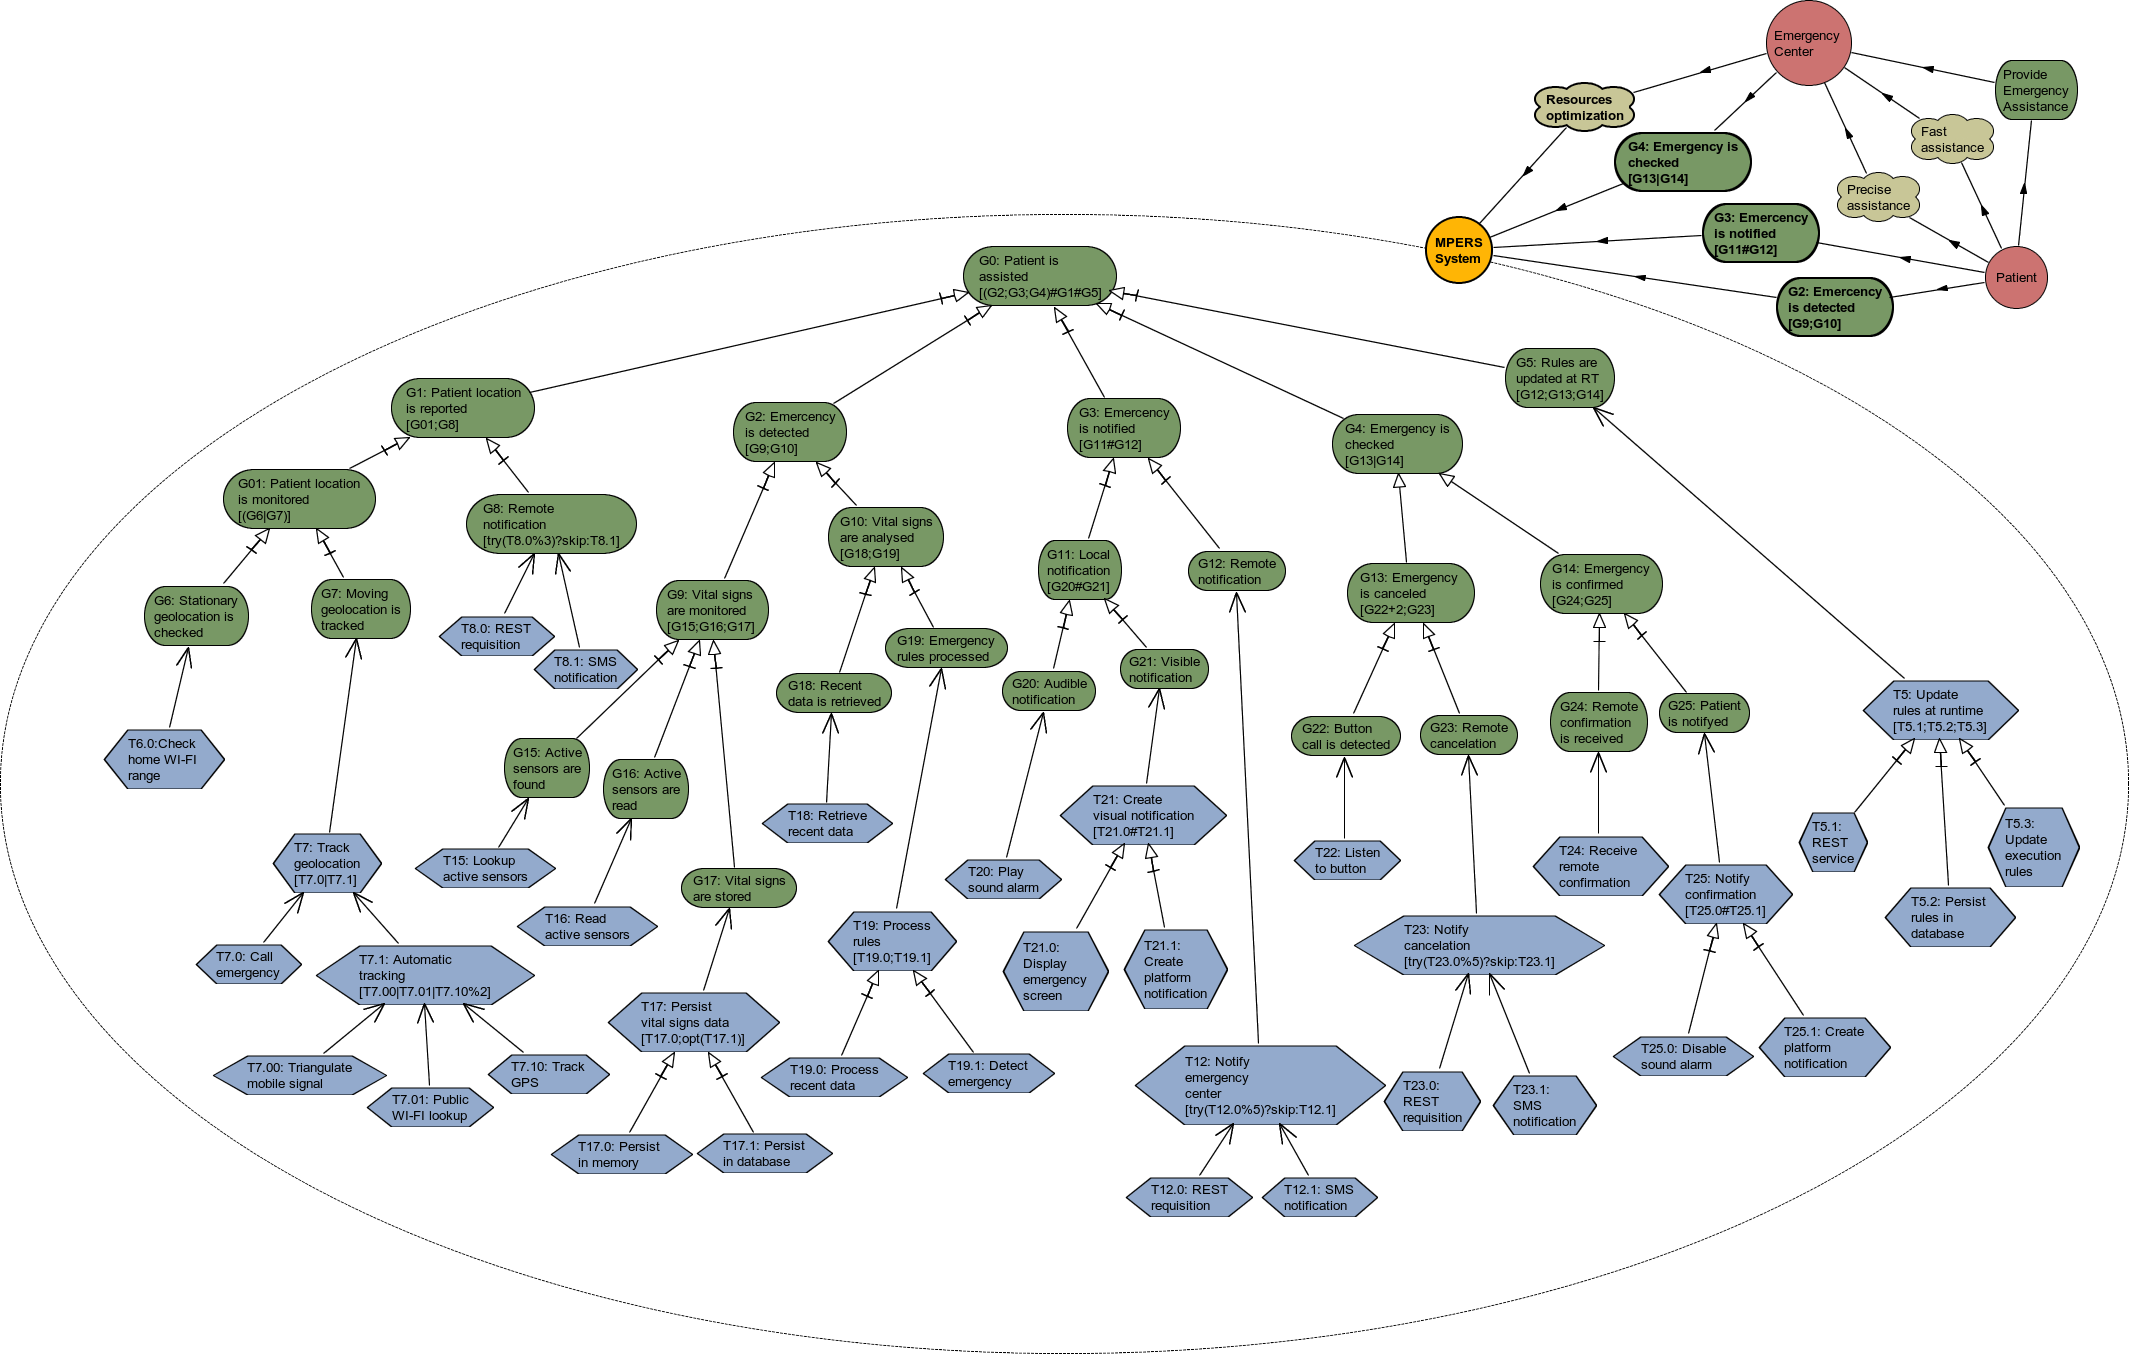
\includegraphics[width=1\textwidth]{imgs/MPERS_LR.png}
\caption{MPERS at TROPOS early requirements phase}
\label{fig:MPERS_LR}
\end{figure*}

Later requirements phase concentrates the analysis in the system-to-be and its operational environment. The MPERS goal model occupies the most part of the diagram and each of its main goals are further decomposed through AND/OR decomposition. Also, means-end decomposition specifies how leaf-goals can be fulfilled by tasks performed by the system actor. Figure~\ref{fig:MPERS_LR} illustrates the late requirements diagram for the MPERS.

To evaluate our proposal, we have explored the PMC technique for the reliability analysis of a system goal model resulting from the TROPOS late requirements phase with additional behaviour and contextual specifications described in the next subsections. The idea is to initially evaluate the approach in a monolithic representation without the additional complexity of a multi-agent architecture. Hence, the evaluation involving later TROPOS phases should be explored in future work. 

%The remaining of this section will focus on the proposed goal-oriented contextual dependability analysis.

%and the runtime regex across goals and tasks specifies dynamic properties of the system-to-be behaviour. 

\subsection{Runtime Goal Modelling}

%stage of the methodology
At this point, the system is modelled as a monolithic actor and its goal model may be extended with the behaviour specification to compose a RGM. This extended model merges multiple views in the same diagram: goals, tasks and relations represent the requirements view for the system-to-be as well as the intentionality behind then, while the runtime specification provides the behaviour specification required for our goal-oriented dependability analysis based on PMC. 

The late requirements diagram in Figure~\ref{fig:MPERS_LR} already presents the runtime regex. Goals and tasks in the model have been notated with an unique identifier (ID). Numeric IDs are prefixed with an `G', in the case of goals, and `T', in the case of tasks. For each decomposed element, a corresponding runtime regex consisting of IDs and rules specifies the behaviour of all immediately underlying goals and tasks. Parenthesis are used for grouping related goals/tasks and for clarification purpose only, as temporal order is parsed from the type of the rule and its position in the regex.

RGM behaviour specification rules have been described in Chapter~\ref{ch:baseline}. The following subsection compares the MPERS RGM presented in Figure~\ref{fig:MPERS_LR} to a UML activity diagram for better understanding of the model and its specified behaviour.

%in terms of goal achievement  and task execution.


\subsubsection{RGM - UML activity diagram comparison}\label{ssec:RGM-UML}

A similar behaviour specification achieved with the RGM in Figure~\ref{fig:MPERS_LR} could be provided by an UML activity diagram with activities representing the leaf-tasks in the model. However, activity diagrams have an homogeneous abstraction level and do not clearly correlate behaviour to the requirements they are meant to satisfy. In contrast to the RGM, activity diagrams denote behaviour through graphical symbols, while the RGM mixes the original goal model notation with a runtime regex. This simple notation increases the utility of a goal model diagram. Figure~\ref{fig:MPERS_UMLAD} presents an activity diagram corresponding to the MPERS leaf-tasks. 

\begin{figure*}[h!]
\centering
\includegraphics[width=1\textwidth]{imgs/MPERS_UMLAD.png}
\caption{MPERS tasks represented by a UML activity diagram}
\label{fig:MPERS_UMLAD}
\end{figure*}

Among its limitations, RGM does not express that an emergency has to be confirmed after a time (clock) or signal event as the UML activity diagram does. Both necessary and sufficient conditions for the triggering and fulfilment of goals, tasks and dependencies are provided by Formal TROPOS specification language.  Still, sequential, interleaved, alternative, optional and conditional execution flows as well as multiple executions of the same task can be expressed by the RGM, providing a rich behaviour specification for the system-to-be.

%could be checked for non-functional requirements such as dependability attributes.

The idea of a runtime goal model is not to replace UML activity diagrams, but to complement the static goal model with a clear runtime syntax that could be used for 
documentation, team communication and for conformance verification at both design time - e.g., through model-based verification - and during system execution - as the execution monitoring originally proposed by Dalpiaz et al~\cite{Dalpiaz:2013}. Depending on the complexity of the behaviour specification, a more robust runtime syntax would have to be employed or complemented by traditional UML behaviour models. In this work, RGM is used as input for our goal-oriented dependability analysis based on PMC.

\subsection{Contextual Goal Modelling}

At this phase, the analysis of the environment in which the system will operate is performed. A careful investigation of what is static and what may change during operation should list the contexts facts and variables that may potentially affect goals, operational means (tasks) and the quality of different means (alternatives). In CGM, contexts are be described by statements and facts. Statements must be supported by facts, while facts can be monitored by the system. In our work, we simplify the analysis by just considering context facts. Facts are specified as boolean expressions composed of variables and operators. Variables can hold boolean or real numbers. The following operators can be used in the modelling environment:
%TODO CHECK THE CGM CONTEXT ANALYSIS TO SEE IF FACTS ARE RESTRICTED TO TRUE OR FALSE

\begin{itemize}

\item $<$, $<=$, $>=$, $>$ (relational operators)
\item $=$,\ $!=$ (equality operators)
\item $!$ (negation)
\item $\&$ (conjunction)
\item $|$ (disjunction)
%\item $-$ (unary minus)
%\item $*$, $/$ (multiplication, division)
%\item $+$, $-$ (addition, subtraction)

\end{itemize} 

Table~\ref{tab:MPERS_CTXS} presents the contexts affecting the MPERS system. Each context has an unique identifier (CID), a textual description and the corresponding boolean expression that later will be parsed into a PRISM language formula and compose a guard condition in leaf-tasks modules, as detailed in Section~\ref{ssec:ctx_effects_dtmc}.

% Please add the following required packages to your document preamble:
% \usepackage{booktabs}
\begin{table}[h]
{\renewcommand{\arraystretch}{1.5}
\footnotesize
\begin{tabularx}{\textwidth}{@{}lllX@{}}
\toprule
\textbf{CID} & \textbf{Description} & \textbf{Boolean expression}                          	&\textbf{A.E.}\\ \midrule
\textbf{C1}  & User is at home      & $HOME\_WIFI\quad \&\quad LOCATION\_AGE\ <=\ 10$ 	&G6\\
\textbf{!C1}  & User is out         & $!HOME\_WIFI\quad |\quad LOCATION\_AGE\ >\ 10$	&G7\\
\textbf{C2}  & Mobile signal        & $SERVICE\ !=\ false$                           	&T8.1\\
\textbf{C3}  & WI-FI is on          & $WIFI\ !=\ false$                              	&T6.0. T7.01\\
\textbf{C4}  & GPS signal           & $GPS\ !=\ false$                               	&T7.10\\
\textbf{C5}  & Internet             & $INTERNET\ !=\ false$                          	&T8.0, T12.0\newline T23.0, G5\\
\textbf{C6}  & Disk space available & $DISK\_SPACE\ >=\ 5$                           	&T17.1\\
\textbf{C7}  & Low health risk      & $HR\ =\ 1$                                     	&G13\\
\textbf{C8}  & Moderate health risk & $HR\ =\ 2$                                     	&-\\
\textbf{C9}  & Severe health risk   & $HR\ =\ 3$                                     	&-\\
\textbf{C10} & Emergency            & $EMERGENCY\ !=\ false$                                         	&G5\\ \bottomrule
\end{tabularx}
\caption{Contexts affecting the MPERS system.}
\label{tab:MPERS_CTXS}
}
\end{table}
\normalsize

Column A.F. (Affected element) indicates one or more goals/tasks that are activated/restricted by the context. Isolated boolean facts have been explicitly specified using the \textit{false} term just for clarification. In order to specify the context effects in the modelling environment, we have used the formal specification area for each affected element provided by the TAOM4E GORE tool, as presented by Figure~\ref{fig:TAOM4E_CTX_CREATION}.

\begin{figure*}
\centering
\includegraphics[width=1\textwidth]{imgs/TAOM4E_CTX_CREATION.png}
\caption{Context effect associated in the TAOM4E formal specification area.}
\label{fig:TAOM4E_CTX_CREATION}
\end{figure*}

%TODO IN CONTEXT SECTION
%For all these environment variables, a context analysis as proposed by Ali et al. may be employed for the creation of the rationale for context monitoring, i.e., for how each context condition may be asserted as true or false through the monitoring of environment information. Some contexts are mapped to single monitorable facts, like `GPS signal' and `battery life'. Other like `patient health risk' are composed of multiple facts in a propositional formula.


%The multiple context effects described in 

%To evaluate our verification approach with the MPERS case study, we have used a discrete-time Markov chain (DTMC) probabilistic model and focused on the verification of NFR related to dependability, i.e., NFR that are either direct attributes encompassed by dependability or that are related to one or more of these attributes.

%\subsection{Non-functional requirements analysis}
%
%%\subsubsection{NFR framework with quantitative constraints}
%
%TROPOS goal model also provides rationale for NFR analysis, as it originally inherited the softgoal analysis from the NFR framework~[NFR]. In our approach, non-functional constraints are modelled as qualitative hard goals with a clear cut value for its satisfaction, complementing the other NFRs modelled as softgoals. As a benefit of a goal-oriented modelling for NFRs, the elicitation of a given NFR may be justified by its relation to other elements in the model. Figure~\ref{fig:MPERS_NFR} presents the NFRs for the MPERS system actor.
%
%\begin{figure*}[h!]
%\centering
%\includegraphics[width=1\textwidth]{imgs/MPERS_NFR.png}
%\caption{MPERS non-functional requirements.}
%\label{fig:MPERS_NFR}
%\end{figure*}
%
%%Intersting for motivation!
%Similarly to the Awareness Requirements by Souza et al.~\cite{Souza:2011}, some NFR define metrics over other requirements. These meta-requirements are not directly fulfilled by system functionalities like `emergency awareness' is fulfilled by `notify emergency' or `confidentiality' could be fulfilled by `user authentication', but by how these functionalities will perform. Reliability, for instance, is inversely proportional to the likelihood of failures. Hence, the reliability metric depends on the probability of system functionalities to successfully meeting their goals. 
%
%Other MPERS NFR are `emergency awareness' and `resources optimization'. These softgoals are addressed by system functionalities. The former receives a full contribution (double positive sign) from goal `emergency is notified', meaning it is fully satisfied by this goal. The later is just assumed to be partially satisfied by the `emergency is checked' functional goal.
%
%
%%The conformity to these NFR is not implicit in the model, it requires some verification technique.
%
%%PUT a goal model with hard goal NFRs!
%
%%PUT SOME NFR CONCEPTUAL MODEL HERE!
%
%Each requirement in a goal model must come from another requirement through decomposition, means-end or contribution links, or it must be directly mapped to stakeholder needs through dependency links. Emergency center attended the patient's needs by providing and maintaining the MPERS system itself and by assuring other NFR for the system. 
%
%Reliability was selected as metric over the system execution (meta-requirement), while availability and maintainability are partially satisfied by the `low power consumption' softgoal and MPERS ability to update emergency rules at runtime, respectively. This proposal focus on reliability analysis and will not discuss the verification of other relevant NFRs.
%
%%evaluation will focus on the reliability metric and, for the sake of simplicity, will omit the verification of other relevant NFRs.

\section{Goal-oriented Probabilistic Verification Model}\label{ssec:NFR-verification}

%NOT HERE!
%The probabilistic verification of systems with variability is not a novelty by itself. Many proposals have addressed this problem in the context of Dynamic Software Product Lines (DSPL), some of then using the PMC technique~[Vini, Paula, Who Else?]. In DSPL, optional and alternative features may be activated or deactivated at runtime. A family based verification of one or multiple NFRs, also called qualitative goals, indicates what combinations are valid or which combination is optimal.

This section describes the application of PMC technique for the reliability verification of a runtime goal model with additional context effect notations. We call it a goal-oriented probabilistic verification or goal-oriented dependability analysis because the probabilistic model, in this case a DTMC model, is built directly from a runtime goal model with the purpose of evaluating PCTL properties related to the probability of different goals in being fulfilled, i.e., to the dependability of the system.

% to verify the conformance of the RGM to defined non-functional constraints and also to solve the variability problem at design time considering both cases explained in Section~\ref{sec:variability}, i.e., for static context and dynamic contexts.

\subsection{Leaf-tasks as DTMC modules}

To demonstrate the well-formation of our transformation from a RGM to a DTMC model, we use the transition system definition from the computer science theory. A transition system $TS$ is formally defined by the tuple $(S, Act, \rightarrow, I, AP, L)$, where:

\begin{itemize}

\item $S$ is a set of states,
\medskip

\item $Act$ is a set of actions,
\medskip

\item $\rightarrow\ \subset\ S\ x\ Act\ x\ S$ is a transition system,
\medskip

\item $I\ \subseteq\ S$ is a set of initial states,
\medskip

\item $AP$ is a set of atomic propositions, and
\medskip

\item $L:\ S\rightarrow2^{AP}$ is a labelling function.

\end{itemize}

$TS$ is called finite if $S$, $Act$, and $AP$ are finite. An action $\alpha$ evolves the system from state $s$ to $s\squote$ if $(s, \alpha, s\squote)\ \in\ \rightarrow$, $\{s, s\squote\}\ \subseteq\ S$ and $s$ is the current state. In case a state has more than one outgoing transition, the `next' transition is chosen nondeterministically. Labels relates a set $L(s)\ \in 2^{AP}$ of atomic propositions to any state $s$. Given a propositional logic formula $\Phi$, then $s\ \models\ \Phi\ \iff\ L(s)\ \models\ \Phi$~\cite{Baier:2008}.

We present the resulting transition system for one or more tasks after the application of each behaviour rule in terms of states and actions that causes state transitions. One important aspect is the simultaneity of the transitions in different tasks states, as some transitions are synchronized for different purposes, while others are interleaved or sequential in time. The objective is to demonstrate how the $RGM\ \rightarrow\ DTMC$ transformation preserves the semantics of the RGM behaviour specification.

Once the transition system resulting from a behaviour rule has been clearly defined, the corresponding DTMC part is presented. In our proposal, leaf-tasks are mapped to DTMC modules in PRISM language. Leaf-tasks have their execution states mapped to a module variable whose values belongs to $S$ from the corresponding transition system $TS$. In specific, the states $s \in S$ are:

%From the RGM original set of goal/tasks instance states, we considered the following values:
%
%\subsection{Leaf-tasks as DTMC modules}
%
%The MPERS RGM in Figure~\ref{fig:MPERS_LR} expands its main goals in further subgoals that are ultimately satisfied by operational tasks, which in turn can also be expanded in more granular subtasks until the leaf-tasks. In the DTMC model, leaf-tasks have their execution states mapped to a module variable (sT15 variable in Figure~\ref{fig:PRISM_TSK_MODULE}). From the RGM original set of goal/tasks instance states, we considered the following values:

\begin{itemize}

\item Initial(s=0): corresponds to the initial/ready state of a given leaf-task. From this state, a transition may occur to the running state, if this task is part of a system alternative to be analysed, or directly to the final success state, if the opposite.
\medskip

\item Running(s=1): corresponds to the execution state of a given leaf-task. From this state, a transition to the final success or failure states may occur. A variable ranging from 0 - 1 defines the task's reliability, i.e., the probability of a transition to the success state - and the complementary transition probability to the failure state (variable rTask15 in Figure~\ref{fig:PRISM_TSK_MODULE}).
\medskip

\item Success(s=2): corresponds to the absorbing and final success state of a singular task execution.
\medskip

\item Skipped(s=3): indicates that a task does not participate in the fulfilment of the analysed goal and should not impact the analysis results.
\medskip

\item Failure(s=4): the opposite from the final success state, meaning that a singular task execution has failed.

\end{itemize}

Figure~\ref{fig:UML_TSK_STATES} illustrate leaf-tasks' states in a UML state diagram.

%, while Figure~\ref{fig:PRISM_TSK_MODULE} presents a system task as a PRISM module.

%TODO refactor image and include skipped state
\begin{figure*}[ht!]
\centering
\includegraphics[width=0.8\textwidth]{imgs/UML_TSK_STATES.png}
\caption{State diagram for leaf-tasks in the DTMC module.}
\label{fig:UML_TSK_STATES}
\end{figure*}

%PRISM modules are containers for variables and commands, i.e., for states and behaviour

%\begin{figure*}[ht]
%\centering
%\includegraphics[width=1\textwidth]{imgs/PRISM_TSK_MODULE.png}
%\caption{A PRISM DTMC module representing T15 (mandatory) task.}
%\label{fig:PRISM_TSK_MODULE}
%\end{figure*}


%init (0), running (1), success (2) and failure (3). Success and failure are the final absorbing states for a task instance. Transition to these states is conditioned to the rTask probability: the closer this variable is to 1, the higher the probability of reaching the success state. 


\subsection{Building the high-level DTMC model from a RGM}

%The state-based verification of non-functional constraints that specifies how different functionalities should perform is a complex task that involves a representation of system states and their transitions. A goal model may define system requirements with variable abstraction levels. As such, the feasibility of the verification of a given metric depends on the information provided by the model.

The conventional goal model defined by the TROPOS methodology will be called design-time goal model (DGM) in contrast to the RGM. A DGM is formally defined as a directed graph $M = (I, R)$, where $I$ is a set of intentional elements (nodes), while $R$ is a set of relations (edges). For simplification purposes, we consider only goals and tasks as intentional elements, and limit the relations to AND/OR-decompositions, i.e., intentional elements can be in one of the two disjoint refinement groups: AND-nodes and OR-nodes. A goal refined by AND/OR tasks is called leaf-goal, while a leaf-task has no further refinements.

%The first step in building a DTMC from a RGM is parsing the behaviour rules. 

Given a DGM $M = (I, R)$, a RGM is built by associating each non-leaf element $\epsilon \in I$ with an expression $annot(\epsilon)$, called a behaviour annotation that is intended to specify the behaviour of the decomposed subgoals/tasks of $\epsilon$. The only trivial case are single means-end tasks, whose behaviour is inherit from their leaf-goal. All goals and tasks elements in the model receive an unique identifier $ID(\epsilon)=prefix(\epsilon) + counter(\epsilon)$, where $prefix()$ returns a $G$ or a $T$ for goals and tasks, respectively, and $counter()$ returns an unique positive integer in the goals set, if $type(\epsilon)=Goal$, or a repetition of the leaf-goal positive integer with further decimals to identify a tasks and its refinements. Figure~\ref{fig:RGM_REGEX} illustrates the identifiers for a leaf-goal, for its trivial means-end task and for this task's refinements, as well as its behaviour annotation.

\begin{figure*}[ht!]
\centering
\includegraphics[width=0.45\textwidth]{imgs/RGM_REGEX.png}
\caption{Goal $G_{17}$ decomposed by task $T_{17}$ that is refined by subtasks $T_{17.0}$ and $T_{17.1}$.}
\label{fig:RGM_REGEX}
\end{figure*}

%Numeric IDs are prefixed with an `G', in the case of goals, and a `T', in the case of tasks. For each decomposed element, a corresponding runtime regex consisting of IDs and rules specifying the behaviour of all immediately underlying goals and tasks. Parenthesis are used for grouping related goals/tasks and for clarification purpose only, as temporal order is parsed from the type of the rule and its position in the regex.

%In the DTMC models for PMC verification of system behaviour, activities have their execution time mapped to discrete values. For instance, in a system workflow, initial activities start at a given time slot, e.g., zero. Considering the the following activities to only start after all previous activities are finished, 

Given a goal $G_i \in I$ and a set $\Lambda$ of leaf-tasks that fulfils the branches of subgoals until $G$, where $\Lambda \subset I$, a DTMC model for $G$ is composed of $k=|\Lambda|$ modules with leaf-tasks states, actions and transitions. This model must represent, in its finite state abstraction, the same behaviour of the corresponding RGM, i.e., it must preserve goals/tasks temporal order and other behaviour semantics specified by the runtime regex. We call the resulting verification model of a high-level DTMC because leaf-tasks are similar to activities in a high-level UML diagram whose behaviours could be further detailed, e.g., by sequence diagrams. 

%We are not interested in checking system instance conformance to its runtime goal model through monitoring as the original RGM proposal. We focus on the estimation of non-functional metrics based on the high-level DTMC model. 

To improve the understanding of the activities workflow described by the DTMC model, we have used a time abstraction formalized by the tuple $\tau = (s,b)$, where $s$ represents a discrete time slot and $p$ a time branch. The RGM starts in $\tau = (0,0)$ and is parsed following a depth first sequence. Whenever two intentional elements are in sequential time order, they are in subsequent time slots, i.e., $\tau_i = (s,b) \Rightarrow \tau_{i+1} = (s+1, b)$. Elements annotated with interleaved order are in the same time slot, but in different time branches, i.e., $\tau_i = (s,b) \Rightarrow \tau_{i+1} = (s, b+1)$. The time slot and branch of any mapped leaf-task in the DTMC model defines if they are interleaved to other tasks or if their execution is prior or subsequent to other tasks in the model.

%Accordingly, tasks originated from interleaved decompositions follows different execution branches.

%Each leaf-task in the DTMC model starts at a discrete time slot. Time slots maps the sequence order of tasks executions. To differentiate the time of parallel tasks, time path is incremented by interleaved task executions, while time slot is incremented by sequential executions. 

Next, each RGM rule is detailed within three levels: an UML activity diagram representation, the resulting transition system (formal demonstration) and the DTMC model described in PRISM language.

%the representation of RGM rules in DTMC modules are presented, as well as the increment in the time slot and time path caused by each rule as illustrated by corresponding UML activity diagrams.

%The following subsections describe each of the RGM rules with additional UML activity diagrams to illustrate the resulting behaviour on the execution of system leaf-tasks that are later mapped to a probabilistic verification model in Section~\ref{ssec}. The \textit{slot} and \textit{path} notations refers to discrete time abstractions in a DTMC model as it will be explained in Section~\ref{ssec:RGM-UML}.


\subsubsection{Sequential order}

Two fundamental behaviour rules consist of the temporal orders for the fulfilment of goals and execution of tasks. In a RGM, the `;' and `\#' symbols represent sequential and parallel temporal orders, respectively. Figures~\ref{fig:UML_SEQ_TSKS} and~\ref{fig:UML_PAR_TSKS} illustrate this behaviours in UML activity diagrams.

\begin{figure}[ht!]
        \centering
        \begin{subfigure}[b]{0.4\textwidth}
                \includegraphics[width=\textwidth]{imgs/UML_SEQ_TSKS.png}
				\caption{Sequential tasks T1;T2.}
				\label{fig:UML_SEQ_TSKS}
        \end{subfigure}        
        \quad %\quad, \qquad, \hfill
        \begin{subfigure}[b]{0.4\textwidth}                
                \includegraphics[width=0.85\textwidth]{imgs/UML_PAR_TSKS.png}
				\caption{Interleaved tasks T1\#T2.}
				\label{fig:UML_PAR_TSKS}
        \end{subfigure}%
          
\end{figure}

Sequential tasks ($T1;T2$) have subsequent time slots, meaning that T2's execution is subsequent to T1's execution. To model this, we have synchronized T2's initial transition to T1's final transition (refer to Figure~\ref{fig:UML_TSK_STATES} for a state diagram). Considering the transition systems $TS_1$ and $TS_2$ corresponding to T1 and T2: $TS_i\ =\ (S_i, Act_i, \rightarrow_i, I_i, AP_i, L_i),\ 1 <= i <= 2$, the transition system resulting from $TS_1;TS_2$ is defined by: 

$$Act_1 \cap Act_2\ =\ \{\alpha\},\quad \frac{s_1\ \xrightarrow{\alpha}\ s\textquotesingle_1\ \wedge\ s_2\ \xrightarrow{\alpha}\ s\textquotesingle_2}{<s_1,s_2>\ \xrightarrow{\alpha}\ <s_1\textquotesingle, s_2\textquotesingle>}$$

\noindent
where $s_1 = running$, $s\textquotesingle_1 = success$, $s_2 = initial$, $s\textquotesingle_2 = running$ and $\alpha = success_1$.
\medskip

%$$Post(s_{running},\alpha)\ =\ \{s_{success}\},\ s \in S_1,\quad Post(s_{initial},\alpha)\ =\ \{s_{running}\},\  s \in S_2.,$$

In contrast, interleaved tasks ($T1\#T2$) have their initial state transition synchronized at the same time slot, but occupy different time paths, i.e., following state transitions of these tasks are interleaved. In this case, the transition system resulting from $TS_1\#TS_2$ following a previous transition system $TS_p$ is defined by:

$$Act_p\ \cap\ Act_1 \cap Act_2\ =\ \{\alpha\},\quad \frac{s_1\ \xrightarrow{\alpha}\ s\textquotesingle_1\ \wedge\ s_2\ \xrightarrow{\alpha}\ s\textquotesingle_2}{<s_1,s_2>\ \xrightarrow{\alpha}\ <s_1\textquotesingle, s_2\textquotesingle>}$$

\noindent
where $s_1 = initial$, $s_2 = initial$, $s\textquotesingle_1 = running$, $s\textquotesingle_2 = running$ and $\alpha = success_p$, and:

$$\beta_1 \in Act_1,\ \beta_2 \in Act_2,\quad \frac{s_1\ \xrightarrow{\beta_1}\ s\textquotesingle_1}{<s_1,s_2>\ \xrightarrow{\beta_1}\ <s\textquotesingle_1, s_2>},\quad \frac{s_2\ \xrightarrow{\beta_2}\ s\textquotesingle_2}{<s_1,s_2>\ \xrightarrow{\beta_2}\ <s_1, s\textquotesingle_2>}$$

\noindent
where $s_1 = running$, $s_2 = running$, $ s\textquotesingle_1 = success$, $s\textquotesingle_2 = success$ and $\beta_i = success_i$.
\bigskip

Generically, for any finite number of interleaved tasks succeeding a task $T_0$, a resulting transition system $TS_0;TS_1\#..\#TS_i\#..\#TS_N$, where $0 < i \leq N$ is defined as:

%General interleaving
$$\bigcap_{0 \leq i \leq N} Act_i\ =\ \{\alpha\},\quad \frac{s_0\ \xrightarrow{\alpha}\ s\textquotesingle_0\ \wedge\ ...\ \wedge\ s_i\ \xrightarrow{\alpha}\ s\textquotesingle_i\ \wedge\ ...\ \wedge\ s_N\ \xrightarrow{\alpha}\ s\textquotesingle_N}{<s_0,...,s_i,...,s_N>\ \xrightarrow{\alpha}\ <s_0\textquotesingle, ...,s_i\textquotesingle,...,s_N\textquotesingle>}$$
\medskip

\noindent
where $s_i = initial$, $s\textquotesingle_i = running$ and $\alpha = success_0$, and:

$$\bigcup_{0 < i \leq N} \frac{s_i\ \xrightarrow{\beta_i}\ s\textquotesingle_i}{<s_1,...,s_i,...s_N>\ \xrightarrow{\beta_1}\ <s_1, ..., s\textquotesingle_i, ..., s_N>}$$
\medskip

\noindent
where $s_i = running$, $ s\textquotesingle_i = success$, $\beta_1 \in Act_i$  and $\beta_i = success_i$. Listings~\ref{lst:PRISM_SEQ_TSKS} and~\ref{lst:PRISM_INT_TSKS} present the PRISM DTMC modules for $T15;T16$ and $T21.0\#T21.1$, respectively.
\medskip

\begin{lstlisting}[language=Prism, caption={Sequential tasks T15 and T16 as DTMC modules with final transitions of the first module synchronized to the initial transition of the second.},label={lst:PRISM_SEQ_TSKS}] 
const double rTaskT15;
module T15_LookupActiveSensors
	sT15 :[0..4] init 0;
	
	[success0_0]  sT15 = 0 -> (sT15'=1);//init to running	
	[] sT15 =  1 -> rTaskT15 : (sT15'=2) + (1 - rTaskT15) : (sT15'=4);//running to final state
	[success0_1] sT15 = 2 -> (sT15'=2);//final state success
	[success0_1] sT15 = 3 -> (sT15'=3);//final state skipped
	[failT15] sT15 = 4 -> (sT15'=4);//final state failure
endmodule

const double rTaskT16;

module T16_ReadActiveSensors
	sT16 :[0..4] init 0;
	
	[success0_1]  sT16 = 0 -> (sT16'=1);//init to running	
	[] sT16 =  1 -> rTaskT16 : (sT16'=2) + (1 - rTaskT16) : (sT16'=4);//running to final state
	[success0_2] sT16 = 2 -> (sT16'=2);//final state success
	[success0_2] sT16 = 3 -> (sT16'=3);//final state skipped
	[failT16] sT16 = 4 -> (sT16'=4);//final state failure
endmodule
\end{lstlisting}

\begin{lstlisting}[language=Prism, caption={Interleaved tasks T21.0 and T21.1 as DTMC modules with initial transitions synchronized and running transitions interleaved.},label={lst:PRISM_INT_TSKS}] 
const double rTaskT21_0;

module T21_0_DisplayEmergencyScreen
	sT21_0 :[0..4] init 0;
	
	[success0_7] G2 &  sT21_0 = 0 -> (sT21_0'=1);//init to running
	[] sT21_0 =  1 -> rTaskT21_0 : (sT21_0'=2) + (1 - rTaskT21_0) : (sT21_0'=4);//running to final state
	[success1_8] sT21_0 = 2 -> (sT21_0'=2);//final state success
	[success1_8] sT21_0 = 3 -> (sT21_0'=3);//final state skipped
	[failT21_0] sT21_0 = 4 -> (sT21_0'=4);//final state failure
endmodule

const double rTaskT21_1;

module T21_1_CreatePlatformNotification
	sT21_1 :[0..4] init 0;
	
	[success0_7] G2 &  sT21_1 = 0 -> (sT21_1'=1);//init to running
	[] sT21_1 =  1 -> rTaskT21_1 : (sT21_1'=2) + (1 - rTaskT21_1) : (sT21_1'=4);//running to final state
	[success2_8] sT21_1 = 2 -> (sT21_1'=2);//final state success
	[success2_8] sT21_1 = 3 -> (sT21_1'=3);//final state skipped
	[failT21_1] sT21_1 = 4 -> (sT21_1'=4);//final state failure
endmodule
\end{lstlisting}

%Other supported behaviours are: alternative execution ($E1|E2$), optional execution (opt(E1)) and conditional execution (try(E)?E1:E2). For alternative execution,

\subsubsection{Alternative execution}

In the case of OR-decomposition with additional `|' behaviour rule, a resulting XOR-decomposition specifies that only one goal/task among two or more may be selected, i.e., they are mutually exclusive. Figures~\ref{fig:UML_ALT_TSKS} illustrate the alternative OR-decomposition in an UML activity diagram.

\begin{figure*}[ht!]
\centering
\includegraphics[width=0.35\textwidth]{imgs/UML_ALT_TSKS.png}
\caption{\detokenize{Alternative tasks T1|T2.}}
\label{fig:UML_ALT_TSKS}
\end{figure*}

Alternative execution is conditioned to some input data provided by the analyst, at design time, or by the system, at runtime. Considering the transition systems $TS_1$ and $TS_2$ corresponding to alternative tasks T1 and T2: $TS_i\ =\ (S_i, Act_i, \rightarrow_i, I_i, AP_i, L_i),\quad 1\ \leq\ i\ \leq\ 2$, the transition system resulting from $TS_1|TS_2$ is defined by the same sequential/interleaved rules and by additional rules for the transitions from the initial state to the running or to the skipped states: 

$$\{\gamma_1, \gamma_2\}\ \subset\ (Act_1\ \cap\ Act_2)$$

$$\frac{s_1\ \xrightarrow{\gamma_1}\ s\textquotesingle_1\ \wedge\ s_2\ \xrightarrow{\gamma_1}\ s\textquotesingle_2}{<s_1,s_2>\ \xrightarrow{\gamma_1}\ <s\textquotesingle_1, s\textquotesingle_2>},\quad \frac{s_1\ \xrightarrow{\gamma_2}\ s\textquotesingle\textquotesingle_1\ \wedge\ s_2\ \xrightarrow{\gamma_2}\ s\textquotesingle\textquotesingle_2}{<s_1,s_2>\ \xrightarrow{\gamma_2}\ <s\textquotesingle\textquotesingle_1, s\textquotesingle\textquotesingle_2>}$$
\medskip

\noindent
where $s_1 = initial$, $s_2 = initial$, $s\textquotesingle_1 = running$, $s\textquotesingle_2 = skipped$, $s\textquotesingle\textquotesingle_1 = skipped$, $s\textquotesingle\textquotesingle_2 = running$, $\gamma_1 = select_1$ and $\gamma_2 = select_2$. 
\medskip

Generically, for any finite number of alternative tasks, a resulting transition system $TS_1|..|TS_i|..|TS_N$, for $0 < i \leq N$, is defined as:

$$\{\gamma_1,..,\gamma_i,..,\gamma_N\}\ \subset\ \bigcap_{0 < i \leq N} Act_i$$

$$\bigcup_{0 < i \leq N} \frac{s_1\ \xrightarrow{\gamma_i}\ s\textquotesingle_1\ \wedge\ ...\ \wedge\ s_i\ \xrightarrow{\gamma_i}\ s\textquotesingle_i\ \wedge\ ...\ \wedge\ s_N\ \xrightarrow{\gamma_i}\ s\textquotesingle_N}{<s_1,...,s_i,...s_N>\ \xrightarrow{\gamma_i}\ <s\textquotesingle_1, ..., s\textquotesingle_1, ..., s\textquotesingle_N>}$$
\medskip

\noindent
where $s_i\ =\ initial,$ for $0\ <\ i\ \leq\ N$, $s\textquotesingle_j\ =\ skipped$ and $\gamma_j\ =\ skip$ for $0\ <\ j\ \leq\ N$, $j\ \neq\ i$, $s_i\ =\ running$ and $\gamma_i\ = select$.
\bigskip

To represent this rule in a DTMC model, an additional parameter  defines which alternative from a set of two or more is selected for analysis. Instead of different actions for selecting different alternatives ($\{select_1, select_2,..\}$), alternative selection is achieved by guard conditions on the transitions to the running/skipped states of each module. Listing~\ref{lst:PRISM_ALT_TSKS} presents the DTMC modules for alternative tasks T7.00, T7.01 and T7.10. For this behaviour rule, both time slot and time path are equal for the alternatives, as only one task may be selected.
\medskip

\begin{lstlisting}[language=Prism, caption={Alternative tasks T7.00, T7.01 and T7.10 as DTMC modules with additional integer variable used for selection.},label={lst:PRISM_ALT_TSKS}] 
const int XOR_T7_00_T7_10_T7_01=0;
const double rTaskT7_00;

module T7_00_TriangulateMobileSignal
	sT7_00 :[0..4] init 0;
	
	[success0_0] XOR_T7_00_T7_10_T7_01=0 & sT7_00 = 0 -> (sT7_00'=1);//init to running
	[success0_0] XOR_T7_00_T7_10_T7_01!=0 & sT7_00 = 0 -> (sT7_00'=3);//not used, skip running
	[] sT7_00 =  1 -> rTaskT7_00 : (sT7_00'=2) + (1 - rTaskT7_00) : (sT7_00'=4);//running to final state
	[success0_1] sT7_00 = 2 -> (sT7_00'=2);//final state success
	[success0_1] sT7_00 = 3 -> (sT7_00'=3);//final state skipped
	[failT7_00] sT7_00 = 4 -> (sT7_00'=4);//final state failure
endmodule

const double rTaskT7_01;

module T7_01_PublicWI_FILookup
	sT7_01 :[0..4] init 0;
	
	[success0_0] XOR_T7_00_T7_10_T7_01=1 & sT7_01 = 0 -> (sT7_01'=1);//init to running
	[success0_0]  XOR_T7_00_T7_10_T7_01!=1 & sT7_01 = 0 -> (sT7_01'=3);//not used, skip running	
	[] sT7_01 =  1 -> rTaskT7_01 : (sT7_01'=2) + (1 - rTaskT7_01) : (sT7_01'=4);//running to final state
	[success0_1] sT7_01 = 2 -> (sT7_01'=2);//final state success
	[success0_1] sT7_01 = 3 -> (sT7_01'=3);//final state skipped
	[failT7_01] sT7_01 = 4 -> (sT7_01'=4);//final state failure
endmodule

const double rTaskT7_10;

module T7_10_TrackGPS
	sT7_10 :[0..4] init 0;
	triesT7_10 : [0..2] init 0;

	[success0_0] XOR_T7_00_T7_10_T7_01=2 & sT7_10 = 0 -> (sT7_10'=1);//init to running
	[success0_0]  XOR_T7_00_T7_10_T7_01!=2 & sT7_10 = 0 -> (sT7_10'=3);//not used, skip running
	[] sT7_10 =  1 -> rTaskT7_10 : (sT7_10'=2) + (1 - rTaskT7_10) : (sT7_10'=4);//running to final state
	[success0_1] sT7_10 = 2 -> (sT7_10'=2);//final state success
	[success0_1] sT7_10 = 3 -> (sT7_10'=3);//final state skipped
	[failT7_10] sT7_10 = 4 -> (sT7_10'=4);//final state failure
endmodule
\end{lstlisting}

\subsubsection{Optional execution}

Given a decomposed goal or task, its fulfilment or execution may be optional, meaning that at least one other goal/task must necessarily be fulfilled/executed. Figure~\ref{fig:UML_OPT_TSK} illustrate an optional task T.

\begin{figure*}[ht!]
\centering
\includegraphics[width=0.3\textwidth]{imgs/UML_OPT_TSK.png}
\caption{\detokenize{Optional task T.}}
\label{fig:UML_OPT_TSK}
\end{figure*}

Considering the transition systems $TS_o\ =\ (S_o, Act_o, \rightarrow_o, I_o, AP_o, L_o)$ corresponding to an optional tasks $opt(T)$, $TS_o$ is defined by the same sequential/interleaved rules and by the additional rules:

$$\{\gamma_1,\gamma_2\}\ \subset\ Act_o$$

$$\frac{s_o\ \xrightarrow{\gamma_1}\ s\textquotesingle_o}{<s_o>\ \xrightarrow{\gamma_1}\ <s\textquotesingle_o>},\quad \frac{s_o\ \xrightarrow{\gamma_2}\ s\textquotesingle\textquotesingle_o}{<s_o>\ \xrightarrow{\gamma_2}\ <s\textquotesingle\textquotesingle_o>}$$
\medskip

\noindent
where $s_o = initial$, $s\textquotesingle_o = running$, $s\textquotesingle\textquotesingle_o = skipped$, $\gamma_1 = select_o$ and $\gamma_2 = skip_o$.
\medskip

To avoid a deadlock in case of a skipped optional task, the initial transition of subsequent tasks is synchronized to both succeed and skip actions, resulting in the following rule for $TS_o;TS$:

$$\{\alpha, \gamma\}\ \subset\ (Act_o\ \cap\ Act_1)$$

$$\frac{s_o\ \xrightarrow{\gamma}\ s\textquotesingle_o\ \wedge\ s\ \xrightarrow{\gamma}\ s\textquotesingle}{<s_o, s>\ \xrightarrow{\gamma}\ <s\textquotesingle_o, s\textquotesingle>}$$
\medskip

\noindent
where $s_o = running$, $s\textquotesingle_o = success$, $s = initial$, $s\textquotesingle = running$, $\gamma = skip_o$ and  $\alpha = succeed_o$.
\medskip

$$\frac{s_o\ \xrightarrow{\alpha}\ s\textquotesingle_o\ \wedge\ s\ \xrightarrow{\alpha}\ s\textquotesingle}{<s_o, s>\ \xrightarrow{\alpha}\ <s\textquotesingle_o, s\textquotesingle>}$$
\medskip

\noindent
where $s_o = initial$, $s\textquotesingle_o = skiped$, $s = initial$ and $s\textquotesingle = running$.
\medskip

Similarly to alternative execution, optional tasks are enabled for analysis by an additional variable in the model. Instead of different actions, as described by the transition system $TS_o$, the select variable ($OPT\_17\_1$ in Listing~\ref{lst:PRISM_OPT_TSK}) determines in a single action (run) which state will follow the initial state: running, if $OPT\_T\_ID=1$, or skipped, if $OPT\_T\_ID=0$. Optional tasks does increment the time slot or path according to the previous temporal order rule. Listing~\ref{lst:PRISM_OPT_TSK} illustrates the DTMC module for optional task T17.1. 
\medskip

\begin{lstlisting}[language=Prism, caption={An optional task T17.1 as a DTMC module with additional select variable OPT\_T17\_1.},label={lst:PRISM_OPT_TSK}] 
const double rTaskT17_1=0.999;
const int OPT_T17_1;

module T17_1_PersistInDatabase
	sT17_1 :[0..4] init 0;
	
	[success1_3] sT17_1 = 0 -> (OPT_T17_1) : (sT17_1'=1) + (1 - OPT_T17_1) : (sT17_1'=3);//init to running or to final skipped
	[success1_3] sT17_1 = 0 -> (sT17_1'=4);//init to fail
	[runT17_1] sT17_1 =  1 -> rTaskT17_1 : (sT17_1'=2) + (1 - rTaskT17_1) : (sT17_1'=4);//running to final state
	[success1_4] sT17_1 = 2 -> (sT17_1'=2);//final state success
	[success1_4] sT17_1 = 3 -> (sT17_1'=3);//final state skipped
	[failT17_1] sT17_1 = 4 -> (sT17_1'=4);//final state failure
endmodule
\end{lstlisting}

\subsubsection{Conditional execution}

Some goals/tasks are conditioned to the fulfilment/execution of another goal/task. In such cases, an OR-decomposition is annotated with a ternary rule $try(E1)\ ?\ E2:E3$ where $E2$ is conditioned to the success of $E1$, while $E3$ is conditioned to its failure. The $skip$ term is used if no further behaviour is conditioned to either the success or the failure of $E1$, for instance, in $try(T1)?skip:T2$, where task $T2$ is only required for execution if $T1$ fails and no further behaviour is expected if $T1$ succeeds. The $try(E1)\ ?\ E2:E3$ pattern specifies a fault tolerant behaviour. Figure~\ref{fig:UML_TRY_TSKS} illustrate a conditional decomposition.

\begin{figure*}[ht!]
\centering
\includegraphics[width=0.60\textwidth]{imgs/UML_TRY_TSKS.png}
\caption{\detokenize{Optional task T.}}
\label{fig:UML_TRY_TSKS}
\end{figure*}

Considering the transition systems $TS_1$, $TS_2$ and $TS_3$ corresponding to alternative tasks T1, T2 and T3: $TS_i\ =\ (S_i, Act_i, \rightarrow_i, I_i, AP_i, L_i),\quad 1\ \leq\ i\ \leq\ 3$, the transition system resulting from $try(TS_1)\ ?\ TS_2:TS_3$ is defined by the same sequential/interleaved rules and the additional rules for conditional transitions from the initial state to the running/skipped states: 

$$\{\delta_1, \delta_2\}\ \subset\ (Act_1\ \cap\ Act_2 \cap\ Act_3)$$

$$\frac{s_1\ \xrightarrow{\delta_1}\ s\textquotesingle_1\ \wedge\ s_2\ \xrightarrow{\delta_1}\ s\textquotesingle_2\ \wedge\ s_3\ \xrightarrow{\delta_1}\ s\textquotesingle_3}{<s_1,s_2, s_3>\ \xrightarrow{\delta_1}\ <s\textquotesingle_1, s\textquotesingle_2, s\textquotesingle_3>},\quad \frac{s_1\ \xrightarrow{\delta_2}\ s\squote\squote_1\ \wedge\ s_2\ \xrightarrow{\delta_2}\ s\squote\squote_2\ \wedge\ s_3\ \xrightarrow{\delta_2}\ s\squote\squote_3}{<s_1, s_2, s_3>\ \xrightarrow{\delta_2}\ <s\squote\squote_1, s\squote\squote_2, s\squote\squote_3>}$$
\medskip

\noindent
where $s_1 = initial$, $s_2 = initial$, $s_3 = initial$, $s\textquotesingle_1 = success$, $s\textquotesingle_2 = running$, $s\textquotesingle_3 = skipped$, $s\squote\squote_1 = failure$, $s\squote\squote_2 = skipped$, $s\squote\squote_3 = running$, $\delta_1 = success_1$ and $\delta_2 = failure_1$. 
\medskip

In the DTMC model, shared actions synchronize the execution of conditional tasks to the success and failure of a third task. Figure~\ref{lst:PRISM_TRY_TSKS} present the DTMC module for conditional tasks T9.0 and T9.1. 
\medskip

Any task subsequent to a conditional execution must have its initial transition synchronized to all possible outcomes, i.e., given the transition system $try(TS_1)\ ?\ TS_2:TS_3;TS_4$, the additional rule applies:

$$\alpha_2\ \in\ (Act_2\ \cap\ Act_4),\quad \alpha_3\ \in\ (Act_3\ \cap\ Act_4)$$

$$\frac{s_2\ \xrightarrow{\alpha_2}\ s\textquotesingle_2\  \wedge\ s_4\ \xrightarrow{\alpha_2}\ s\textquotesingle_4}{<s_2, s_4>\ \xrightarrow{\alpha_2}\ <s\textquotesingle_2, s\textquotesingle_4>},\quad \frac{s_3\ \xrightarrow{\alpha_3}\ s\textquotesingle_3\  \wedge\ s_4\ \xrightarrow{\alpha_3}\ s\textquotesingle_4}{<s_3, s_4>\ \xrightarrow{\alpha_3}\ <s\textquotesingle_3, s\textquotesingle_4>}$$
\medskip

\noindent
where $s_2 = running$, $s_3 = running$, $s_4 = initial$, $s\textquotesingle_2 = success$, $s\textquotesingle_3 = success$, $s\textquotesingle_4 = running$, $\alpha_2 = success_2$ and $\alpha_3 = success_3$. 
\medskip

\begin{lstlisting}[language=Prism, caption={Conditional tasks T9.00 and T9.1 as DTMC modules.},label={lst:PRISM_TRY_TSKS}] 
const double rTaskT9_0=0.999;

module T9_0_RESTRequisition
	sT9_0 :[0..4] init 0;
	
	[success0_2] sT9_0 = 0 -> (sT9_0'=1);//init to running
	[] sT9_0 =  1 -> rTaskT9_0 : (sT9_0'=2) + (1 - rTaskT9_0) : (sT9_0'=4);//running to final state
	[success2_3] sT9_0 = 2 -> (sT9_0'=2);//final state success
	[success2_3] sT9_0 = 3 -> (sT9_0'=3);//final state skipped
	[failT9_0] sT9_0 = 4 -> (sT9_0'=4);//final state failure
endmodule

const double rTaskT9_1=0.999;

module T9_1_SMSNotification
	sT9_1 :[0..4] init 0;
	
	[failT9_0]  sT9_1 = 0 -> (sT9_1'=1);//init to running
	[success2_3] sT9_1 = 0 -> (sT9_1'=3);//not used, skip running
	[] sT9_1 =  1 -> rTaskT9_1 : (sT9_1'=2) + (1 - rTaskT9_1) : (sT9_1'=4);//running to final state
	[success2_4] sT9_1 = 2 -> (sT9_1'=2);//final state success
	[success2_4] sT9_1 = 3 -> (sT9_1'=3);//final state skipped
	[failT9_1] sT9_1 = 4 -> (sT9_1'=4);//final state failure
endmodule
\end{lstlisting}

%For alternative, optional and conditional execution of leaf-tasks, the final skipped state ($s_i\squote=skipped=3$) has a deterministic loop triggered by the same action form the final success state ($s_i\squote=success=2$), namely $success2\_4$ in Listing~\ref{lst:PRISM_TRY_TSKS}. This is justified by the fact that a skipped task is not not a failed task. Hence, it must not block the execution of subsequent task(s) whose initial transition(s) is(are) synchronized to the success action of previous task(s).

\subsubsection{Cardinality}

Variations of the original RGM proposal was employed for the $E+$ and $E\#$ cardinality rules. Instead of an infinite/undetermined number of goal/task instances, analyst should provide the exact number of instances for goals achievements and tasks executions. This information is required for the generation of the DTMC verification model from a runtime goal model. Figures~\ref{fig:UML_MUL_SEQ_TSKS} and \ref{fig:UML_MUL_PAR_TSKS} respectively illustrate sequential and interleaved task behaviours.

\begin{figure}[ht!]
        \centering
        \begin{subfigure}[b]{0.3\textwidth}
                \includegraphics[width=1\textwidth]{imgs/UML_MUL_SEQ_TSKS.png}
				\caption{Sequential executions of task T.}
				\label{fig:UML_MUL_SEQ_TSKS}
        \end{subfigure}        
        \quad %\quad, \qquad, \hfill
        \begin{subfigure}[b]{0.4\textwidth}                
                \includegraphics[width=1\textwidth]{imgs/UML_MUL_PAR_TSKS.png}
				\caption{Interleaved executions of task T.}
				\label{fig:UML_MUL_PAR_TSKS}
        \end{subfigure}%
          
\end{figure}

In our proposal, cardinality is represented by the number of sequential ($E+n$) or interleaved ($E\#n$) executions of the same task. Considering a transition system TS, cardinality follows the same rules of a sequential or interleaved execution, except that only one task is involved. Thus, the resulting transition systems $TS+N$ and $TS\#N$ are the same as $TS_1;..;TS_i;..;TS_N$ and $TS_1\#..\#TS_i\#..\#TS_N$, where: 

$$\sum_{i=1}^{N-1} TS_{i}=TS_{i+1}$$.

To represent these rules in a DTMC model, the corresponding leaf-tasks modules are repeated $n - 1$ times though PRISM language module renaming, as $n=1$ is trivially represented by the original module. In the case of sequential cardinality, the state variable, the initial and final transition actions are renamed for all repetitions, forming an execution chain of the same task. In the case of interleaved cardinality, only the state variable is renamed, synchronizing the initial and the final actions of the repeated modules, but leaving the run actions unsynchronized, forming an interleaved execution order of the same task. Increments to the time slot is multiplied by the cardinality $n$, in the case of sequential execution, and limited to $1$, in the case of interleaved execution.

Listings~\ref{lst:PRISM_MUL_SEQ_TSKS} and \ref{lst:PRISM_MUL_INT_TSKS} present the DTMC modules for both cases. The second example does not come from the MPERS RGM in Figure~\ref{fig:MPERS_LR} and was introduced to exemplify the interleaved cardinality module renaming approach.
\medskip

%or by interleaved transitions with PRISM language module renaming, in the case of interleaved execution ($E\#n$). In the first case, only after $n$ unsuccessful retries, a transition to the failure state occurs. In the second case, $n$ simultaneous transitions from the initial state to the running state occurs before interleaved transitions from the running state to the final success/failure state may happen. The failure label is also renamed to avoid deadlocks if one or more of the interleaved tasks fails.


\begin{lstlisting}[language=Prism, caption={Sequential cardinality with n=2 for task T22.},label={lst:PRISM_MUL_SEQ_TSKS}] 
const double rTaskT22;
module T22_ListenToButton
	sT22 :[0..4] init 0;	

	[success0_8] sT22 = 0 -> (sT22'=1);//init to running
	[] sT22 =  1 -> rTaskT22 : (sT22'=2) + (1 - rTaskT22) : (sT22'=4);//running to final state
	[success0_9] sT22 = 2 -> (sT22'=2);//final state success
	[success0_9] sT22 = 3 -> (sT22'=3);//final state skipped
	[failT22] sT22 = 4 -> (sT22'=4);//final state failure
endmodule
module T22_S2 = T22_ListenToButton [ sT22=sT22_S2, success0_9=success0_10, success0_8=success0_9 ] endmodule
\end{lstlisting}
\medskip

\begin{lstlisting}[language=Prism, caption={Interleaved cardinality with n=3 for task T22.},label={lst:PRISM_MUL_INT_TSKS}] 
const double rTaskT22;
const double maxRetriesT22=2;
module T22_ListenToButton
	sT22 :[0..4] init 0;
	
	[success0_8]  sT22 = 0 -> (sT22'=1);//init to running
	[] sT22 = 1 -> rTaskT22 : (sT22'=2) + (1 - rTaskT22) : (sT22'=4);//running to final state
	[success0_9] sT22 = 2 -> (sT22'=2);//final state success
	[success0_9] sT22 = 3 -> (sT22'=3);//final state skipped
	[failT22] sT22 = 4 -> (sT22'=4);//final state failure
endmodule
module T22_N2 = T22_ListenToButton [ sT22_N2=sT22, rTaskT22_N2=rTaskT22 ] endmodule
module T22_N3 = T22_ListenToButton [ sT22_N3=sT22, rTaskT22_N3=rTaskT22, failT22_N2=failT22] endmodule
\end{lstlisting}

%Listing~\ref{ls:MPERS_DTMC} presents the DTMC model for the MPERS.

In addition to the original RGM, we also support the specification of retries for tasks executions ($E@n$) as a sort of cardinality behaviour rule. In this particular case, before a failure may occur, the \textit{run} action is performed multiple times until the maximum number of retries or the final success state are reached. In the first case, a second action takes the task module to the final failure state. Listing~\ref{lst:PRISM_MUL_RTRY_TSKS} illustrates this behaviour in a DTMC module.

\begin{lstlisting}[language=Prism, caption={Retry behaviour with n=2 for task T22.},label={lst:PRISM_MUL_RTRY_TSKS}] 
const double rTaskT22;
const double maxRetriesT22=2;
module T22_ListenToButton
	sT22 :[0..4] init 0;
	triesT22 : [0..2] init 0;	
	
	[success0_3]  sT22 = 0 -> (sT22'=1);//init to running
	[] sT22 = 1 & triesT22 < maxRetriesT22 -> rTaskT22 : (sT22'=2) + (1 - rTaskT22) : (triesT22'=triesT22+1);//try
	[] sT22 = 1 & triesT22 = maxRetriesT22 -> (sT22'=4);//no more retries
	[success0_4] sT22 = 2 -> (sT22'=2);//final state success
	[success0_4] sT22 = 3 -> (sT22'=3);//final state skipped
	[failT22] sT22 = 4 -> (sT22'=4);//final state failure
endmodule
\end{lstlisting}

%Given a transition system $TS$, the transition system resulting from $TS@n$ is defined by the same sequential/interleaved rules and by the additional rules for 

%To illustrate our proposal for NFR verification of a single alternative, we selected the local goal G5 that defines the state where emergency rules are updated without major system interruption. Table~\ref{tab:MPERS_NFR} has a non-functional constraint for this goal that specifies the minimum

In Table~\ref{tab:MPERS_DTMC_SLOTS}, the final settings for the time slot, branch and other dynamic aspects of leaf-tasks parsed from the RGM and used for the generation of a DTMC model are presented.

% Please add the following required packages to your document preamble:
% \usepackage{booktabs}
\begin{table}
{\renewcommand{\arraystretch}{1.5}
\begin{tabularx}{\textwidth}{@{}lllllll@{}}
\toprule
\textbf{Task}  & \textbf{Time path} & \textbf{Time slot} & \textbf{Optional} & \textbf{Conditional} & \textbf{Alternative} & \textbf{Cardinality} \\ \midrule
\textbf{T15}   & 0                  & 0                  & false             & false                & false                & 1           \\
\textbf{T16}   & 0                  & 1                  & false             & false                & false                & 1           \\
\textbf{T17.0} & 0                  & 2                  & false             & false                & false                & 1           \\
\textbf{T17.1} & 0                  & 3                  & \textbf{true}    & false                 & false                & 1           \\
\textbf{T18}   & 0                  & 4                  & false             & false                & false                & 1           \\
\textbf{T19.0} & 0                  & 5                  & false             & false                & false                & 1           \\
\textbf{T19.1} & 0                  & 6                  & false             & false                & false                & 1           \\
\textbf{T20}   & 0                  & 7                  & false             & false                & false                & 1           \\
\textbf{T21.0}   & 1                & 7                  & false             & false                & false                & 1           \\
\textbf{T21.1}   & 2                & 7                  & false             & false                & false                & 1           \\
\textbf{T9.0}  & 3                  & 7                  & false             & false	        		& false                 & 1           \\
\textbf{T9.1}  & 3                  & 7                  & false             & \textbf{S. T9.0}     & false                 & 1           \\
\textbf{T22}   & 0                  & 8                  & false             & false                & \textbf{T24}                  & \textbf{2}  \\
\textbf{T23.0} & 0                  & 9                  & false             & false                & false                  & 1           \\
\textbf{T23.1} & 0                  & 9                  & false             & \textbf{S. T23.0}   & false                  & 1           \\
\textbf{T24}   & 0                  & 8                  & false             & false                & \textbf{T22}                  & 1           \\
\textbf{T25.0} & 0                  & 9                  & false             & false                & \textbf{T25.1                 } & 1           \\
\textbf{T25.1} & 0                  & 9                  & false             & false                & \textbf{T25.0}                  & 1           \\
\textbf{T5.0} & 4                   & 0                  & false             & false                & false                & 1           \\
\textbf{T5.1} & 4                   & 0                  & false             & false                & false                & 1           \\
\textbf{T5.2} & 4                   & 0                  & false             & false                & false                & 1           \\ \bottomrule
\end{tabularx}
\caption{Dynamic aspects of the MPERS leaf-tasks in the DTMC model.}
\label{tab:MPERS_DTMC_SLOTS}
}
\end{table}

\subsection{Context effects in the DTMC model}\label{ssec:ctx_effects_dtmc}

Regarding a goal-oriented dependability analysis based on PMC, context variation may change the scope of the verification and consequently limit the operational leaf-tasks that must be part of the analysis - either because they do not have a goal to satisfy in that context or because they are restricted by that context and cannot be selected for execution. Besides the effects over goals and tasks, we have not considered the direct context effect over qualitative softgoals, but only the indirect effect over the probability of fulfilling different system tasks, as softgoals are not part of our formal analysis.

Given a CGM (in specific, the final goal model becomes a CRGM), all context effects specified in the goal model are parsed. We have also used a depth first approach for traversing the directed tree graph. Even if a context variable occurs multiple times in the same context formula or across other contexts in the model, only one variable is declared in the DTMC model (variable declaration). A reference to this variable is then used to compose identical context formulas as guard conditions in the modules corresponding to the affected leaf-tasks, according to the type of effect it imposes.

%and identical formulas are declared in the high-level DTMC model as guard conditions to the transition from the initial state to the running state

%In the DTMC verification model, context restrictions must follow a computable pattern. 

\subsubsection{Contextual goals activation/restricted}

If a goal is activated/restricted by a given context, the corresponding verification scope must be adjusted. The MPERS RGM in Figure~\ref{fig:MPERS_LR} has a few goals whose activation depends on a specific context condition, as specified in Table~\ref{tab:MPERS_CTXS}. Consequently, they must not affect the analysis results in other contexts.

For instance, the goals `$G_6: stationary\ geolocation\ is\ checked$' and `$G_7: moving\ geolocation\ is\ tracked$' are mandatory subgoals for the `patient location is monitored' goal. The first is activated by the context `user is at home' and the later by the negation of this same context. Analysts have put this restriction to avoid an aggressive geolocation tracking that consumes too much battery when the user is known to be at home. The following formulas specify this restricting context and its negation:

\begin{equation}\label{eq:C1a}
\textbf{C1:}\quad HOME\_WIFI\quad \&\quad LOCATION\_AGE\ <\ 10
\end{equation}

\begin{equation}\label{eq:C1b}
\textbf{!C1:}\quad HOME\_WIFI\quad |\quad LOCATION\_AGE\ >=\ 10
\end{equation}

Home WI-FI BSSID is configured once and stored by the application. If its signal is not in reach for the last 10 minutes, patient is considered to be out. To map these restrictions into the DTMC model, only one PRISM formula were declared and all leaf-tasks related to the affected goals must include C1 (or its negation) as a condition to the inclusion of these tasks in the analysis. A false evaluation of the context formula (or its negation) automatically excludes the related leaf-tasks from the analysis results by forcing a deterministic transition to the skipped final state (sTask=3). Listing~\ref{lst:PRISM_CTX_GOAL} presents the DTMC module of a MPERS leaf-task whose goal is restricted by the context formula in \eqref{eq:C1a}.
\medskip

\begin{lstlisting}[language=Prism, caption={Variable declaration and module representing a leaf-task from a restricted goal.},label={lst:PRISM_CTX_GOAL}]
const double HOME_WIFI;
const double LOCATION_AGE;
const double rTaskT6_0=0.999;

module T6_0_CheckHomeWI_FIRange
	sT6_0 :[0..4] init 0;
	
	[success0_0] (HOME_WIFI & LOCATION_AGE < 10) & sT6_0 = 0 -> (sT6_0'=1);//init to running
	[success0_0] !(HOME_WIFI & LOCATION_AGE < 10) & sT6_0 = 0 -> (sT6_0'=3);//init to skipped


	[] sT6_0 =  1 -> rTaskT6_0 : (sT6_0'=2) + (1 - rTaskT6_0) : (sT6_0'=4);//running to final state
	[success0_1] sT6_0 = 2 -> (sT6_0'=2);//final state success
	[success0_1] sT6_0 = 3 -> (sT6_0'=3);//final state skipped
	[failT6_0] sT6_0 = 4 -> (sT6_0'=4);//final state failure
endmodule
\end{lstlisting}

It is possible to notice that, if $C1$ is evaluated as false, this task goes to the skipped state and does not affect the verification results.

\subsubsection{Tasks restriction}

Regarding the restriction on system tasks (means), all operations depending on a specific system resource considered to be dynamic could be notated with a context restriction. For instance, the context restriction over the communication tasks `$T_{8.0}: REST\ requisition$' and `$T_{8.1}:REST\ service$' (context `internet is available'), over the geolocation tracking tasks `$T_{7.01}: public\ WIFI$' and `$T_{7.10}: track\ GPS$' (contexts `WI-FI is on' and `GPS signal is available') and over the storage task `$T_{17.1}: persist\ in\ database$' (context `disk memory available'). The following boolean formulas represent these contexts: 

\begin{equation}\label{eq:C2}
\textbf{C2:}\quad CONNECTION
\end{equation}

\begin{equation}\label{eq:C3}
\textbf{C3:}\quad WI\_FI
\end{equation}

\begin{equation}\label{eq:C4}
\textbf{C4:}\quad GPS\_SIGNAL
\end{equation}

\begin{equation}\label{eq:C5}
\textbf{C5:}\quad USED\_DISK <= 95
\end{equation}

These formulas follow the same principle from the previous goal restriction formulas. For C5, we considered less than 95\% of the used disk space and not 100\% to avoid instabilities in the operational system. %We have not considered variations in the mobile signal as a restriction to the communication tasks of `SMS notification' and `voice call' or any other technical impediment at this moment. 

In the DTMC model, restricted leaf-tasks have an additional deterministic transition to the failure state guarded by the negation of the corresponding context formula. Consequently, if the formula is evaluated as false, the leaf-task will certainly fail (sTask=4). This is in accordance to the perception that, if a task is required and restricted at the same time, a failure will occur. Listing~\ref{lst:PRISM_CTX_TASK} presents a DTMC model with one restricted MPERS leaf-task.
\medskip

\begin{lstlisting}[language=Prism, caption={Variable declaration and module representing a leaf-task restricted by a context.},label={lst:PRISM_CTX_TASK}] 
const double CONNECTION;//context variable declaration
const double rTaskT9_0=0.999;

module T9_0_RESTRequisition
	sT9_0 :[0..4] init 0;
	
	[success0_2] (CONNECTION != 0) & sT9_0 = 0 -> (sT9_0'=1);//init to running
	[success0_2] !(CONNECTION != 0) & sT9_0 = 0 -> (sT9_0'=4);//init to failure


	[] sT9_0 =  1 -> rTaskT9_0 : (sT9_0'=2) + (1 - rTaskT9_0) : (sT9_0'=4);//running to final state
	[success2_3] sT9_0 = 2 -> (sT9_0'=2);//final state success
	[success2_3] sT9_0 = 3 -> (sT9_0'=3);//final state skipped
	[failT9_0] sT9_0 = 4 -> (sT9_0'=4);//final state failure
endmodule
\end{lstlisting}

\section{Reliability Analysis}

Once a probabilistic verification model is built from a system RGM with additional context effects (CRGM), different PCTL properties may be specified for verification. As part of our goal-oriented dependability analysis, we focus on the reachability property that can be specified by the $\textbf{F}$ temporal operator, indicating that eventually $\varphi$ has to hold:

\begin{equation}\label{eq:PROB_EXISTANCE}
P=?\ [\ F\ (\varphi)\ ]
\end{equation}

The reachability of a final and successful system state defines the reliability of that system, i.e., the probability in fulfilling its root or ultimate goal. Accordingly, the reachability of a partial success state indicates the partial reliability of the system, i.e., the probability in fulfilling one or more of its subgoals. Given a RGM $R_M = (I, R, annot())$ and a set of leaf-tasks $\Lambda \in I$, the scope of the probabilistic verification is defined as:

\begin{itemize}

\item \textit{Global}, if $\Lambda$ is a minimum set composed of the leaf-tasks that satisfies the chain of subgoals up to the root goal $G_{root}$, where $G_{root}\ \in\ I$. 
%For instance, in Table~\ref{tab:MPERS_NFR} reliability is associated to root goal G1.
\medskip

\item \textit{Local}, if $\Lambda$ is a minimum set composed of leaf-tasks that satisfies the chain of subgoals up to a goal $G_x$, where $G_i\ \in\ I$ and $G_i\ !=\ G_{root}$. 
%For instance, in Table~\ref{tab:MPERS_NFR}, power consumption is (locally) associated to goal G2.
\medskip

\end{itemize}



%both qualitative and quantitative analysis may be performed. 

\subsection{Offline analysis}

%Formula verification consist of a qualitative or quantitative evaluation of a time-bounded or unbounded probability specified in PCTL language.

At design-time, analysts may benefit from the rich graphical environment provided by PRISM probabilistic model checker tool. Given a boolean formula specifying the success in fulfilling a specific MPERS goal $G_9$ whose leaf-tasks have been mapped into the DTMC model:

\begin{equation}\label{eq:Gx}
G_{9S}\ =\ (sT15=2\ \&\ sT16=2)\ \&\ (sT17\_0=2\ \&\ (sT17\_1=2\ |\ sT17\_1=3))
\end{equation}

The probability of fulfilling $G_9$, i.e., the reachability of $G_{9S}$ is specified by the following PCTL property:

\begin{equation}\label{eq:PCTLx}
P\ =\ ?\ [\ F\ (G_{9S})]
\end{equation}

Once the reliabilities of the involved leaf-tasks have been collected, the verification of this PCTL property through PRISM \textit{verification feature} reveals the probability in eventually fulfilling the analysed goal. To illustrate this, for a fixed reliability of $0.98$ for all leaf-tasks in $\Lambda$, the probability of fulfilling $G_9$ is evaluated by PRISM as:

$$P_{reach}(G_{9s})=0.929199$$

PRISM also provides the \textit{experiment feature} that automates multiple instances of a model checking. Instead of fixing the value of all constants in the model, one or more constants may range from an initial value to a final value in fixed steps. The experiment creates a series graph and reveals the trend for the analysed property in respect to the input range. For example, by ranging the reliability of tasks $T_{8.0}$ and $T_{7.10}$ from 0 to 1 in steps of 0.1 and leaving all other leaf-tasks reliabilities values fixed in $0.98$ as part of the $G_{1S}$ reachability property~\eqref{eq:PCTLg1s} verification, the experiments produces the composed graphic in Figure~\ref{fig:OFFLINE_EXPERIMENT}.

\begin{equation}\label{eq:G1s}
G_{1S}\ =\ (sT15=2\ \&\ sT16=2)\ \&\ (sT17\_0=2\ \&\ (sT17\_1=2\ |\ sT17\_1=3))
\end{equation}

\begin{equation}\label{eq:PCTLg1s}
P\ =\ ?\ [\ F\ (G_{1S})]
\end{equation}

\begin{figure*}[ht!]
\centering
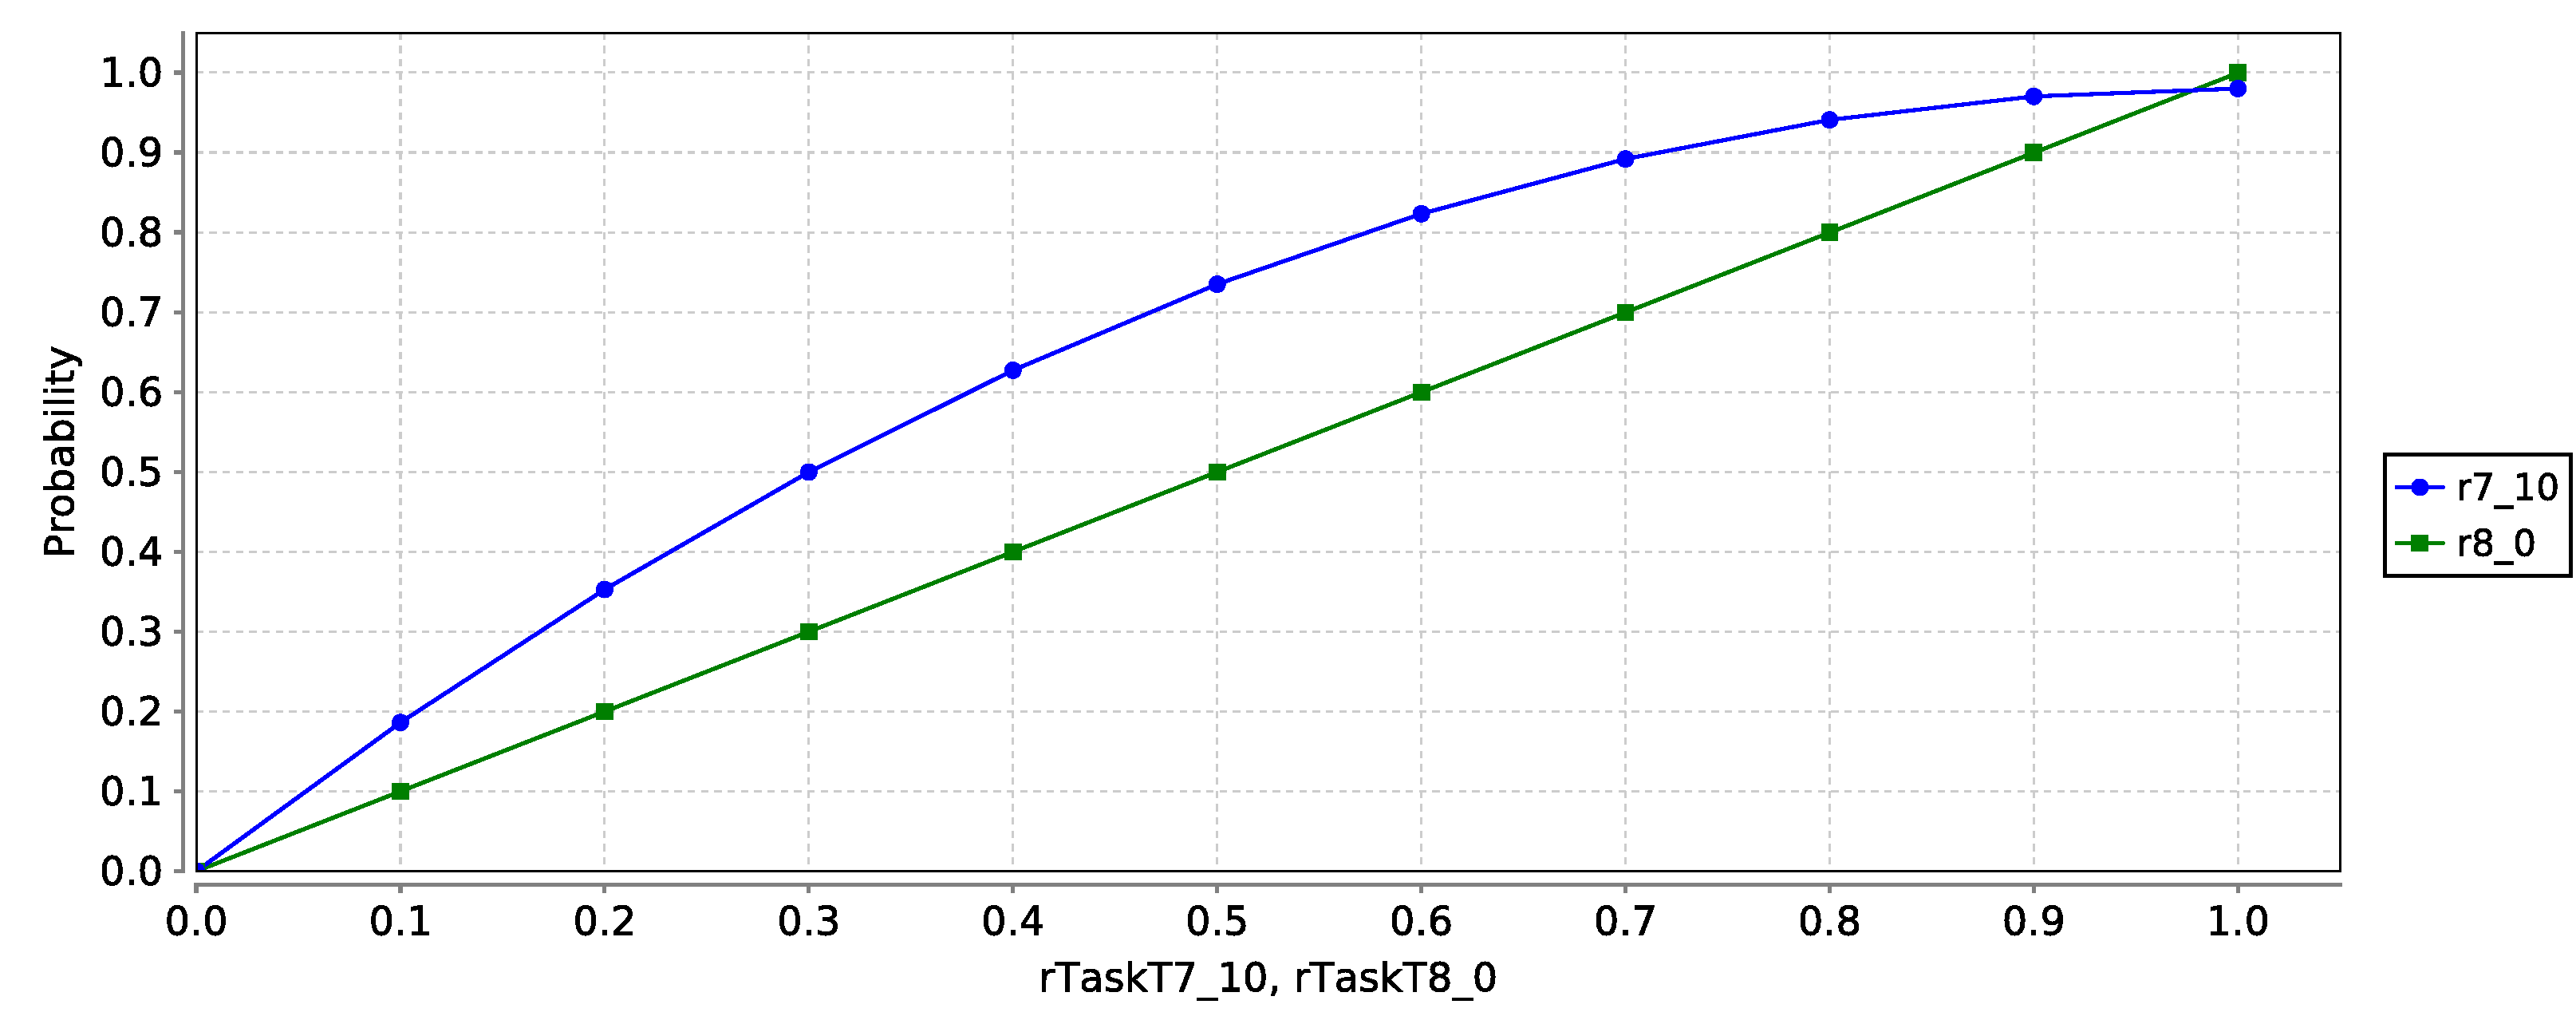
\includegraphics[width=0.80\textwidth]{imgs/OFFLINE_EXPERIMENT.png}
\caption{Experiments results with $T_{7.10}$ and $T_{8.0}$ ranging from 0 to 1.}
\label{fig:OFFLINE_EXPERIMENT}
\end{figure*}

%one property may ask if the probability in fulfilling a given goal G is higher than P. 

\subsubsection{Collecting individual leaf-tasks reliabilities}

Leaf-tasks are not necessarily atomic system operations and are generally described with a high abstraction level. For instance, the MPERS task `Find active sensors' could be further decomposed in more granular and concrete tasks according to the platform, architecture and language used for implementation. 

%As presented in Figure~\ref{fig:MPERS_LR}, MPERS leaf-tasks are not coupled to any platform, architecture and language used for implementation.

%The idea is to leave to analysts the decision concerning the granularity and abstraction level represented by the tasks that will be verified. For instance, the abstract task `find active sensors' could be decomposed in more granular and concrete tasks related to the platform, architecture and language used for implementation. 

The more abstract a task is, the more difficult is to 
obtain their individual metrics - like their reliability, as the trace between an higher-level, abstract activity and the corresponding system operation(s) becomes less evident. For a global evaluation of a given metric, PCM technique requires the individual value for parts involved in the analysed system behaviour, e.g., activities, subactivities or components, depending on what the verification model represents.

In our goal-oriented approach, leaf-tasks are the parts composing a high-level system behaviour representation. Reliability variables define the probability of a successful execution of whatever the leaf-task should perform. To collect this information, analysts may follow a multi-level verification approach. Like in previous works where conventional UML behaviour models are used as input for the creation of a DTMC representation of components interactions, leaf-tasks may also have its behaviour further specified, enabling their individual verification. Figure~\ref{fig:MD_PMC} illustrates this approach.
%TODO cite which are the previous works

\begin{figure*}[ht!]
\centering
\includegraphics[width=0.75\textwidth]{imgs/MD_PMC.png}
\caption{Individual reliabilities of leaf-tasks are estimated through PMC of internal behaviour specification.}
\label{fig:MD_PMC}
\end{figure*}

\subsubsection{Reliability validation}

The probabilistic verification of NFRs, performed as part of the Validation \& Verification (VV) phase in RE, should anticipate violations of non-functional constraints specified for the system-to-be. Treating a detected violation at design time may correspond to actions such as making a different choice for underlying technical components or social actors involved in the execution of tasks, optimizing the behaviour specification or even disposing a violating alternative as a means to satisfy its goal if there is at least one other valid alternative. 

The variability in goal models leads to more than one minimum set of tasks capable of fulfilling local or root goals. In OR-decompositions, at least one alternative is required and the maximum number of combinations is defined by $1 + 2^{(n-1)}$, with n the number of OR-decomposed goals/tasks. Therefore, the verification of all alternatives in a goal model with individual models may prove to be inefficient or infeasible if too many variation points exist in the model.

The PMC approach has already been explored for the verification of other models that supports variability. Rodrigues et al. proposed a family-based verification of software product lines (SPL)~[RODRIGUES]. The main idea is to reduce the analysis effort and boost the feasibility of the SPL verification as parameters in a PRISM probabilistic model generates a single parametric formula for all products in the SPL for a given PCTL property. Individual product evaluation is achieved by the initialization of corresponding parameters in the formula. 

In our proposal, PCM verification follows the same principle of the SPL family-based verification. A parametric DTMC model should be generated from the runtime goal model. Alternatives are selected by passing values to parameters. For instance, if both GPS and triangulation are available means for identifying the patient location, a parameter with values 0 or 1 will indicate which alternative is enabled for verification, as described in Section~\ref{ssec:NFR-verification}.

\subsection{Runtime analysis}

Given a verification model, the feasibility of a runtime analysis depends on metrics such as its scalability and performance and also on the technical feasibility of an automated verification. As part of our third research question, we investigate the use of the PARAM tool to create a parametric formula for the probability of fulfilling one or more system goals in a CRGM.

Despite the similarity to PRISM, as the only additional language term is the \textit{param} keyword used to indicate which variables should be parametrized, PARAM has a few restrictions regarding where parameters can be placed in the model. For example, guard conditions in PRISM language commands cannot be parametrized. In fact, parameters can only be part of the right part of a PRISM command as a transition probability ranging from 0 to 1. This limitation affects the way a leaf-task modules can be built. To address this problem, alternative and optional execution DTMC modules had to be refactored. 

Instead of a single variable indicating which alternative task is selected, multiple variables are employed as the probability in selecting one of the alternatives. As well as in optional execution, a zero value ($XOR\_T_i=0$ or $OPT\_T_i=0$) results in a deterministic transition from the initial state to the skipped state. In opposition ($XOR\_T_i=1$ or $OPT\_T_i=1$), a deterministic transition from the initial state to the running state occurs. We guarantee the structural validity for alternative execution by using a binary construction that avoids more than one alternative to be selected. For instance, the alternative tasks $T_1|..|T_i|..|T_N$ have their initial transition in the following pattern:

\begin{multline}
[success] sT_i = 0 \rightarrow \\ \prod_{j=1;j \neq i}^{N}(1 - XOR\_T_j) * (XOR\_T_i) : (sT_i\squote=1)\ + \\\prod_{j=1;j \neq i}^{N}(XOR\_T_j) * (1 - XOR\_T_i) : (sT_i\squote=3)
\end{multline}

Optional execution also follows this pattern, with $N$ being limited to 1. The remaining behaviour rules are not affected by the guard condition limitation. Nonetheless, the contextual effects are also modelled as guard conditions that defines a deterministic transition to running, skipped or failure state, according the definitions in Section~\ref{ssec:ctx_effects_dtmc}. For this reason, context effects over goals and tasks are not part of the parametric verification model, i.e., this model does not guarantee the structural validity of a CRGM, but only the validity of a RGM. Accordingly, a runtime analysis of a CRGM has to consider the context effects at the formula evaluation time.

Listing~\ref{} presents the parametric formula generated for the reachability property in Eq.~\eqref{eq:PCTLg1s} that specifies the probability in fulfilling the MPERS goal $G_{1}$. 


\subsubsection{Mean-time to failure verification}

The original RGM proposal relies on the assumption that the instance states of goals and tasks can be monitored. In fact, if concrete system operations can be traced back to the leaf-tasks in a RGM, i.e., if an execution trace can be generated indicating the state in which the leaf-tasks instances have been, different statistical measures could be calculated for all the monitored system tasks. For example, the mean-time to failure (MTTF) can be calculated as the average time between failures of a task, i.e., between transitions to their failure state. Disregarding the time to repair (non-repairable system), MTTF defines the reliability of the monitored leaf-tasks. Figure~\ref{fig:MON_PMC} illustrate this approach.

%Accordingly, the success rate of tasks execution, i.e., their reliability, can be extracted by monitoring the system execution trace in controlled executions or in real production environment. 


%and an hybrid approach based on the analysis of the monitored execution trace of system leaf-tasks.

\begin{figure*}[ht!]
\centering
\includegraphics[width=0.75\textwidth]{imgs/MON_PMC.png}
\caption{Individual reliabilities of leaf-tasks are estimated by monitoring their execution.}
\label{fig:MON_PMC}
\end{figure*}

\subsubsection{Reliability analysis for self-adaptive systems}

Considering a parametric formula for the probability in fulfilling one or more system goals and the corresponding values for the individual reliabilities of leaf-tasks, a self-adaptation MAPE loop can enhanced towards dependability with the resulting goal-oriented dependability analysis provided by the evaluation of the formula at runtime.

% in either proving the satisfaction of a reliability constraint for the analysed goal or by 
%In this work we focus on the creation of a parametric, high-level DTMC model corresponding to a runtime goal model with additional context effect notations to enable a goal-oriented reliability analysis for self-adaptive systems. 

As our proposal focus on the runtime reliability analysis for self-adaptive systems and monitoring is already part of a self-adaptation feedback loop, our evaluation with the MPERS case study is based on individual leaf-tasks reliabilities measured through instrumented code execution.

%Each NFR verified by the PMC technique requires corresponding information about individual parts involved in the overall activity, e.g., the reliability, performance, power consumption, cost and other metrics for tasks in a workflow.

%This is a key point in this approach, as it may seen too loose to couple a probabilistic verification to a goal model with a high-level operational representation of a system. But its feasibility becomes more clear if the metrics being verified are compatible with the abstraction level of the leaf-tasks in a specific goal model and individual task metrics are available or can be collected. 

%\subsubsection{Pure model-based approach}
%
%Depending on the purpose of the goal modelling - from early requirements elicitation to detailed design in TROPOS - more granular specification of tasks behaviour can be provided by decomposition and auxiliary UML diagrams. This internal task behaviour specification can be used for individual task analysis of metrics such as reliability and power consumption. 
%
%\subsubsection{Hybrid monitoring approach}
%
%In contrast to a pure model-based verification approach, the hybrid verification requires a concrete system implementation besides the RGM system model. Tasks execution instances could be monitored by instrumented code and the original RMG monitoring algorithms that are able to differentiate one task instance from the other. 
%
%In terms of reliability metric, this approach should be used to collect the frequencies of success and failure of task executions and to calculate their corresponding reliability values used in the high-level DTMC.

\subsection{Specifying non-functional constraints}

The specification of non-functional constraints is a sensible task that depends on both expertise and domain knowledge. For instance, an analyst or a reliability engineer should be aware of what does it mean for a system to be 99.99\% reliable, as this level may not be achieved by any alternative solution and must be coherent to the system criticality - a minor failure consequence could be tolerable, but a catastrophic failure should be avoided by all means. In some cases, the system will have to comply to some industry standards or contract based constraints like in service-oriented computing. Table~\ref{tab:MPERS_NFR} summarizes two possible non-functional constraints for the MPERS.
\medskip

% Please add the following required packages to your document preamble:
% \usepackage{booktabs}
\begin{table}[h]
{\renewcommand{\arraystretch}{1.5}
\begin{tabularx}{\textwidth}{@{}XXX@{}}
\toprule
\textbf{NFR}               & \textbf{Constraint} & \textbf{Target}        \\ \midrule
\textbf{Reliability}       & 99.8\%            & \textbf{G1} \\
\textbf{Power consumption} & 100 p.u.            & \textbf{G2}          \\ \bottomrule
\end{tabularx}
}
\caption{Non-functional metrics for the MPERS system.}
\label{tab:MPERS_NFR}
\end{table}

%softgoals of `continuous assistance' and `correct assistance'

As indicated by the \textit{Target} column, each NFR constraint may be associated to a root level goal or to any of its subgoals. The corresponding probabilistic verification based on the execution of a set of leaf-tasks in the RGM is defined as:

\begin{itemize}

\item \textit{Global}, if the activities set is a minimum set composed of the tasks that satisfies the chain of subgoals up to the root goal $Groot$. For instance, in Table~\ref{tab:MPERS_NFR} reliability is associated to root goal G1.
\medskip

\item \textit{Local}, if the activities set is a minimum set composed of tasks that satisfies the chain of subgoals up to a goal $Gx$, where $Gx != Groot$. For instance, in Table~\ref{tab:MPERS_NFR}, power consumption is (locally) associated to goal G2.
\medskip

\end{itemize}

%put here the formal definition of the root goal, subgoals, activity set, turple, etc

%\subsection{PCTL properties}
%
%The estimation of attributes through PMC technique is limited to those that a probabilistic model may evaluate. Dependability attributes have an abstract definition that must be associated to a concrete and verifiable PCTL property. In this evaluation, we focus on the dependability attribute of reliability. 
%
%Given a DTMC model representing system activities, global reliability may be defined as the probability of reaching a final state where all system goals are achieved. This property is called reachability and can be specified using the PCTL language. For the MPERS root goal G1, reliability can be defined by: $ P=? [ G (noError) ] $, with noError a boolean formula indicating that no task has transitioned to the failure state and P the steady-state probability of a true value for noError formula.


%\begin{itemize}
%
%\item \textbf{Reliability}, represented by the probability of a successful execution of all the activities involved in fulfilling leaf-goals of a certain system alternative. It is also know as the \textit{reachability} as the describes the probability of reaching a final and successful system state. 
%\bigskip
%
%\item \textbf{Availability}, represented by the power consumption estimation to maximize the time that the system will remain operational depending only on its battery. This attribute is well related to mobile computing. 
%\medskip
%
%\end{itemize}



%In Section~\ref{ssec:RGM-UML} we argued that the RGM could replace a corresponding high-level UML activity diagram for PMC verification. However, if internal task behaviour is to be evaluated for a given metric, a both activity and sequence diagrams could serve as input for the evaluation of individual task metrics using a similar PMC technique.

\subsection{Reasoning with Ex-Tropos}



%PMC technique also allows the identification of system alternatives with more influence on each metric through sensitive analysis.

\subsubsection{Solving variability}



\subsubsection{Context selection}

In a contextual goal model, or CGM, contexts may restrict which goals must be achieved, limit the adoptable alternatives (means) and also affect the non-functional metrics of individual tasks. These effects must be considered in a realistic verification. As a novelty, our approach for the verification of non-functional metrics through PMC will also include variable contexts of operation and their effects in the verification model. 

We considered two different approaches for the NFR verification of system with dynamic contexts of operation:

\begin{itemize}

\item \textit{Deterministic context activation, or DCA}: a single context is activated by parameters in the model. In this approach, a parametric formula evaluates a given alternative for a specific context of operation. It is useful for the individual verification of context-alternative pairs, e.g., a context where battery is fully charged and all vital signs sensors are activated.
\medskip

\item \textit{Probabilistic context selection, or PCA}: a probability distribution will define the likelihood of a context to be activated and the corresponding context implications in the verification model to be enabled. It is useful for the emulation of an approximate scenario in which the context of operation varies following some probabilist distribution. The resulting model evaluates an activated alternative for multiple contexts. 

\end{itemize}

Both approaches are complementary as the first verifies the selected alternative for one context at a time and the former verifies a realistic scenario with multiple possible contexts. Table~\ref{tab:SC_DCA_PCA} summarizes each verification approach.

% Please add the following required packages to your document preamble:
% \usepackage{booktabs}
\begin{table}[h]
{\renewcommand{\arraystretch}{2.5}
\begin{tabularx}{\textwidth}{@{}l|XX@{}}
\toprule
			 &                                                         \textbf{Context selection}			 &                                                                                                      \textbf{Alternative selection}			\\ \midrule
\textbf{DCS} & Contexts are individually activated by parameters.  & Alternative selection by the analyst is limited by the activated context.                                                                                    \\
\textbf{PCS} & Context selection follows a probabilistic distribution. & Verification model should select adoptable alternatives according to the activated context.\\ \bottomrule
\end{tabularx}
}
\caption{Description of the different approaches for verifying a system with variable alternatives and variable contexts.}
\label{tab:SC_DCA_PCA}
\end{table}

%If the context selection is deterministic (DCS), there is no reason for verifying an alternative that is known to be incompatible with the selected context. Therefore, only adoptable alternatives must be verified. In opposition, if context selection is probabilistic, that alternative may still be valid in other contexts, hence it must be included in the multi-context evaluation. For instance, the patient location identification through GPS (alternative) will certainly fail if the GPS signal is not available (context). Thus, the DAS-DCS combination checks one compatible context-alternative pair at a time, while DAS-PCS combination leads to the verification of multiple context-alternative pairs at the same time.

The idea behind a probabilistic context selection is to emulate a realistic scenario in which the context of operation varies and the system must avoid requirements violations by  having an adoptable alternative for each context. This holistic evaluation approach provides measures for the validation of self-adaptive systems against non-functional constraints like reliability.

weighted by the probabilistic context distribution. For instance, if GPS signal is available 70\% of the time and triangulation is available 90\% of the time and if each method has its own reliability, namely rGPS and rTRI, the reliability of high-level task `identify patient location' is defined by the expression 0.9*rGPS + 0.1*0.7*rTRI, considering that GPS has priority over triangulation. 

\section{Treating NFR Violations}

\begin{itemize}

\item Making a different choice for underlying components: In some cases the replacement of a technical component for another of the same class can improve the quality of how they achieve their goal. For instance,
\medskip

\item Behaviour optimization: The quality may also depend on the pattern used for the activities execution. The specification of a different pattern may eliminate the non-functional violation. 
\medskip

\item Contextualizing the alternative: An alternative may only violate a NFR in specific contexts. In this case, different valid alternatives may be used according to the context of operation.
\medskip

\item Alternative disposal: If the alternative is in absolute violation or if its validity is restricted to contexts that have at least one other valid alternative, this branch can be eliminated from the model.

\end{itemize}

%Dependability analysis is used to provide information about different dependability attributes related to system failures. These metrics may be specified as non-functional requirements for isolated system functionalities or for the whole system. Instead of softgoals, we use meta-requirements over functional goals with clear-cut quantitative criteria such as `99.999\%' reliable - a probabilistic value to make it compatible with the PMC estimation results.

%To perform the NFR verification, we focus on dependability related metrics that should be estimated and compared to their required constraint values through quantitative analysis. Sensitive analysis to reveal how different system parts contribute to the overall value of those attributes. Sensitive analysis may be considered analogous to the original GORE contribution analysis.



%Eq.~\ref{eq:MPERS_RELIABILITY_FORM} defines the reliability formula for the root goal G1.

%\begin{equation}
%G1r=c^2\label{eq:MPERS_RELIABILITY_FORM}
%\end{equation}

%A family-based PMC is useful for comparing each alternative with non-functional metrics as criteria to decide which one should be used by the system-to-be at design time or by the real system at runtime. At design time, this approach is analogue to the TROPOS contribution analysis. In both cases, a unique parametric formula evaluates a PCTL property corresponding to a non-functional metric.  %improve the example!


% or the verification tool should decide based on some probabilistic distribution setted by the analysts (probabilistic alternative selection, or PAS).

%In contrast, PAS provides verification for systems that include variability in its design. The verification of NFR metrics for these systems depend on how each alternative is selected during system operation.

